% !TEX program = xelatex
% النسخة العربية من «التاريخ الكامل للكون» — مصدر LaTeX
% التحويل إلى PDF:
%   xelatex main.tex && xelatex main.tex
% المتطلبات: محرّك XeLaTeX، حزمة polyglossia، خطّ Amiri (مجلد fonts/ مرفق)،
%             وحزمة fancyhdr وgraphicx وbooktabs وhyperref.
\documentclass[12pt,a4paper,openany]{book}

\usepackage{fontspec}
\usepackage{polyglossia}
\setmainlanguage{arabic}
\setotherlanguage{english}

\newfontfamily\arabicfont[Path=fonts/,Script=Arabic]{Amiri-Regular.ttf}
\newfontfamily\arabicfontsf[Path=fonts/,Script=Arabic]{Amiri-Regular.ttf}
\newfontfamily\arabicfontbf[Path=fonts/,Script=Arabic]{Amiri-Bold.ttf}
\newfontfamily\arabicfonttt[Path=fonts/,Script=Arabic]{Amiri-Regular.ttf}

\usepackage[a4paper,margin=2.4cm]{geometry}
\usepackage{graphicx}
\usepackage{xcolor}
\usepackage{fancyhdr}
\usepackage{booktabs}
\usepackage[hidelinks]{hyperref}

\pagestyle{fancy}
\fancyhf{}
\fancyfoot[C]{\thepage}
\fancyfoot[L]{\footnotesize THE COMPLETE HISTORY OF THE UNIVERSE · ARABIC}
\renewcommand{\headrulewidth}{0pt}

\setlength{\parindent}{1.2em}
\setlength{\parskip}{0.45em}
\linespread{1.35}

\newcommand{\plate}[3]{%
  \begin{figure}[htbp]\centering
    \includegraphics[width=0.92\textwidth,height=0.42\textheight,keepaspectratio]{#1}%
    \par\vspace{0.25em}{\small #2\par}
    \vspace{0.15em}{\footnotesize\textcolor[HTML]{8a5a2b}{المصدر: #3}}
  \end{figure}}

\begin{document}

% ---------- الغلاف ----------
\begin{titlepage}
\centering
\vspace*{2cm}
{\Huge\bfseries التاريخ الكامل للكون\par}
\vspace{0.9cm}
{\Large من الانفجار العظيم إلى ما بعد الزمن\par}
\vspace{0.6cm}
\rule{8cm}{0.6pt}\par
\vspace{0.9cm}
{\large النسخة العربية المنقّحة — ٥٥ تصحيحاً علمياً وتاريخياً\par}
\vspace{0.4cm}
{\normalsize نسخة عربية كاملة · مصوّرة · مبنية على النسخة الإنجليزية المنقّحة\par}
{\normalsize تصحيح علمي موثّق في ٥٥ موضعاً · ١٨ صورةً من أرشيفات الوكالات الأصلية\par}
\vfill
{\footnotesize صُفّت حروفه بخطّ أميري · ١٤٤٧هـ / ٢٠٢٦م\par}
\end{titlepage}

\tableofcontents
\clearpage

% ---------- المقدمة ----------
\chapter*{مقدمة: لماذا نسأل؟}
\addcontentsline{toc}{chapter}{مقدمة: لماذا نسأل؟}

لا يبدأ علمُ الكون من تلسكوب، بل من دهشة. يقف الإنسان على أرضٍ صلبة، فيرى في السماء نقاطاً تتحرك بانتظام، فيسأل: ما هذه؟ ومن أين جاءت؟ وإلى أين تمضي؟ وكلُّ ما بنيناه من فيزياء وفلك إنما هو محاولةٌ طويلة، مؤثّرةٌ في بعض الأحيان، لصياغة هذا السؤال بلغةٍ دقيقة.


هذا الكتاب رحلةٌ واحدة متصلة، لا مجموعةُ فصولٍ منفصلة. يبدأ من اللحظة التي لم يكن فيها «قبل»، ويمرّ بالثانية الأولى، والضوء الأول، والعصور المظلمة، والنجوم الأولى، والموت العنيف للنجوم، وأفق الثقوب السوداء، ثم يعود إلى شمسنا القريبة، وينتهي عند السؤال الذي يفتح كلَّ الأسئلة: ما مصير هذا كله؟


اخترنا الكلمات باقتصاد، لأن كلَّ جملة هنا تحمل رقماً أو نتيجةَ رصدٍ أو تصحيحاً. ولأن النصّ الأصلي خُضع لتدقيقٍ صارم، فإن الأرقام الواردة فيه لا تُذكر للزينة، بل لأنها خلاصة قياس. سنجد في الطريق أرقاماً مذهلة: ١٣٫٧٨٧ مليار سنة، و٢٫٧٢٥ كلفن، و٤٦٫٥ مليار سنة ضوئية، و٣٢٠ إلكترون-فولت-إكسا؛ وكلُّ رقم منها شهادةُ أداةٍ صنعها بشرٌ على أرضٍ صغيرة.


وأخيراً: هذه ليست حكايةً عن الكون بمعزلٍ عنّا. نحن، في كل ذرّة من أجسادنا، أثرٌ كيميائيٌّ لانفجار نجمي قديم؛ وفي كل فكرةٍ من أفكارنا، امتدادٌ لسلسلةٍ من الدهشة بدأت مع أول إنسانٍ رفع رأسه إلى الليل. أن نعرف هو أن نُكمل ما بدأته النجوم: أن نصير وعيَ الكون بذاته، أو على الأقل محاولةً صادقة لبلوغ ذلك.


أما هذه النسخة العربية فقد بُنيت على النصّ الإنجليزي المنقّح، لا على ترجمةٍ حرّةٍ له. وقد تُرجمت الأرقام كما هي، وحُوّلت إلى أرقامٍ عربية-هندية لتُقرأ في سياقها الطبيعي، وضُبطت وحداتها (الكلفن، والفرسخ، والإلكترون-فولت، والسنة الضوئية) ضبطاً موحّداً. وحيث تعارض نصٌّ مع مصدرٍ أوليّ، حُكم للمصدر: بيانات بلانك ٢٠١٨، وقيم مراجعة الجسيمات الأساسية، وثوابت CODATA.


وللصور في هذا الكتاب وظيفةٌ لا تقلّ عن وظيفة النصّ: فهي ليست زينةً تُملأ بها الفراغات، بل شواهدُ رصد. كلُّ صورةٍ هنا مأخوذةٌ من أرشيف الجهة التي أنتجتها — ناسا، ووكالة الفضاء الأوروبية، ومنظمة CERN، وتعاون «تلسكوب أفق الحدث» — ومذيَّلةٌ باسمها في أسفلها. وحيث وُجدت نسختان لموضوعٍ واحد، أُدرجت الاثنتان: إحداهما في الفصل، والأخرى في «ألبوم الصور» في آخر الكتاب.


ويمكن قراءة الكتاب على ثلاثة مستويات: السرد المتّصل لمن يريد الحكاية، والأرقام لمن يريد الدقّة، والصور لمن يريد أن يرى. ومن أراد المستوى الرابع — التحقّق — فسيجد في الخاتمة قائمةً بما صُحّح، وفي الفهرس خطَّاً زمنياً يختصر القصة كلها في صفحةٍ واحدة.


\chapter*{زمنٌ بلا «خارج»: كيف وُلدت فكرة التوسّع}

\addcontentsline{toc}{chapter}{زمنٌ بلا «خارج»: كيف وُلدت فكرة التوسّع}

\markboth{زمنٌ بلا «خارج»: كيف وُلدت فكرة التوسّع}{}


حتى مطلع القرن العشرين، كانت الفيزياء ترى الكون ساكناً أزلياً، بلا بدايةٍ ولا نهاية. لكن تطبيق معادلات النسبية العامة (١٩١٥) على الكون كلّه قاد جورج لومتر، الفيزيائي والكاهن البلجيكي في جامعة لوفان، إلى نتيجةٍ لا مفرّ منها عام ١٩٢٧: الفضاء نفسه لا يستطيع أن يبقى ساكناً.


وإذا عكسنا سهم الزمن في معادلات التوسّع، نصل إلى حالةٍ كان فيها كلُّ المادة والطاقة مضغوطاً في «ذرّةٍ بدائية» بالغة الكثافة والحرارة. سخر فريد هويل من هذه الفكرة فسمّاها «الانفجار العظيم» في برنامجٍ إذاعي عام ١٩٤٩، فصار اللقب الساخر اسماً علمياً.


لكنّ الانفجار العظيم ليس انفجاراً في مكانٍ ما. لا مركز له، ولا حافة، ولا «خارج» يتوسّع فيه. ما يتغيّر هو المسافة المترية بين نقاط الفضاء ذاته؛ فالمجرّات لا تسبح في الفضاء، بل يسبح الفضاء بينها. ولهذا تبدو كلُّ المجرّات مبتعدةً عنّا، لا لأننا في المركز، بل لأن كل نقطةٍ مركزٌ بالنسبة إلى ما حولها.


\plate{images/andromeda-galaxy-hubble-high-resolution--1.jpg}{مجرّة أندروميدا كما رصدها تلسكوب هابل: أقرب مجرّة حلزونية كبيرة، وعلى بعد ٢٫٥ مليون سنة ضوئية تُظهر لنا الانزياحَ الأحمر الذي كشف توسّع الكون.}{ESA/Hubble \& NASA}


والدليلُ المباشر على أن الكون لم يكن موجوداً إلى الأبد يأتي من ظلمة الليل نفسها: لو كان أزلياً وموحّداً بالمجرّات، لانتهى كلُّ خطِّ نظرٍ إلى نجم، ولكان السماء نهاراً دائماً. فظلامُ الليل شهادةٌ كونية على أنّ للكون بداية.


في عام ١٩٢٩ نشر إدوين هابل ورقةً من ست صفحات عدّد فيها مسافات ٢٤ مجرّة، واستنتج أن الانزياح نحو الأحمر يتناسب طردياً مع المسافة. وكانت قيمة ثابته آنذاك ٥٠٠ كيلومتر في الثانية لكل ميغافرسخ، أي أكبر من قيمتها اليوم بنحو سبع مرات. لم يكن هابل مخطئاً في المنهج، بل في معايرة «الشموع القياسية»: فقد خلط بين نجوم السيفيد المتغيّرة وبين عناقيد النجوم الأكثر سطوعاً.


اليوم يبلغ ثابت هابل ٦٧٫٤ كيلومتراً في الثانية لكل ميغافرسخ بحسب بلانك، و٧٣ بحسب قياسات السيفيد والمستعرات من نوع Ia. والفارق بينهما — «توتّر هابل» — لا يتجاوز ٩٪، لكنه يتجاوز حدود الخطأ التجريبي، ولذلك يُعدّ اليوم أحد أهم أسئلة علم الكون.


وثمّة تفصيلٌ يقلب الطريقة التي نقرأ بها الخريطة: الانزياح نحو الأحمر ليس سرعةً في الفضاء، بل تمدّدٌ للفضاء نفسه أثناء انتقال الضوء. فالمجرّة التي نراها على بعد ١٠ مليارات سنة ضوئية لم تكن هناك يوم أُطلق ضوءها؛ لقد كانت أقرب، ثم ابتعدت بفعل التوسّع. أي أن كل صورةٍ كونية هي صورةٌ لزمن، لا لمكان.


في ١٩٩٨، وبينما كان الفلكيون يحاولون قياس تباطؤ التوسّع، فوجئ فريقان مستقلّان بأن المستعرات الأعظم من نوع Ia أبعد مما ينبغي، أي أخفت. الاستنتاج كان مقلقاً: التوسّع يتسارع. نال سول بيرلماتر وبريان شميدت وآدم ريس جائزة نوبل عام ٢٠١١ على هذا الاكتشاف، وسمّينا ما يسبّبه «الطاقة المظلمة» دون أن نعرف ما هي.


وللقياس سلّمٌ لا درجةً واحدة: نبدأ بالعناقيد المتحرّكة (parallax) للنجوم القريبة، ثم السيفيد في مجرّة أندروميدا، ثم المستعرات في المجرّات البعيدة، وأخيراً الخلفية الميكروية. كل درجة تعاير التي تليها، وكل خطأ في درجةٍ ينتقل مضروباً إلى ما بعدها؛ ومن هنا كان ثابت هابل أصعبَ رقمٍ في الفلك.


ومن المفارقات أن أعمق ما نعرفه عن الكون يأتي من أبسط ما نراه: ضوءٌ انزاح نحو الأحمر. فالانزياح z ليس سوى النسبة بين طول الموجة المرصودة والأصلية؛ وعند z = ١ يكون الضوء قد تضاعف طوله، وعند z = ١١٠٠ نصل إلى أول ضوءٍ حرّ في الكون.


\chapter*{الخريطة الأولى: خلفية الكون الميكروية}

\addcontentsline{toc}{chapter}{الخريطة الأولى: خلفية الكون الميكروية}

\markboth{الخريطة الأولى: خلفية الكون الميكروية}{}


في عام ١٩٦٥، التقط أرنو بنزياس وروبرت ويلسون، عن غير قصد، ضجيجاً ميكروياً ثابتاً في كل اتجاه، بعد أن طردا الحمام ونظّفا الهوائي من فضلاته العازلة. ولم يكن ذلك الضجيج عطلاً، بل كان الصدى الحراري لأول لحظات الكون: إشعاعٌ خلفيٌّ ميكروي بدرجة حرارة ٢٫٧٢٥ كلفن، وهو أقدمُ ضوءٍ يمكن رصده.


هذا الضوء انطلق عندما كان عمر الكون ٣٨٠ ألف سنة، حين برد البلازما إلى نحو ٣٠٠٠ كلفن، فاتحدت البروتونات بالإلكترونات وتشكّلت ذرّات الهيدروجين المتعادلة، وأصبح الكون شفافاً للمرة الأولى: لحظة «إعادة الاتحاد».


التقلّبات الدقيقة في درجة حرارة هذه الخريطة، بنسبة واحدٍ من مئة ألف، هي بذور كل شيء: بذور المجرّات والعناقيد والفراغات. قاستها مركبات COBE ثم WMAP ثم بلانك بدقّةٍ جعلت علم الكون علماً قياسياً بالمعنى الحرفي؛ ومن هذه الخريطة وحدها استخرجنا عمر الكون (١٣٫٧٨٧ ± ٠٫٠٢٠ مليار سنة) ونسب مكوّناته: نحو ٤٫٩٪ مادةً عادية، و٢٦٫٨٪ مادةً مظلمة، و٦٨٫٣٪ طاقةً مظلمة.


\plate{images/planck-cosmic-microwave-background-map-e-2.jpg}{السماء كما رصدها مسبار بلانك في تسع نطاقات ترددية: الخلفية الميكروية وتراكمات الغبار والمجرّات، وفي الصفّ الأوسط تُقرأ تقلّبات الحرارة التي وُلدت منها كل البنى.}{ESA / Planck Collaboration}


الخريطة ليست صورةً للسماء فحسب، بل هي أرشيف. كل بقعةٍ زرقاء أبرد قليلاً، وكل بقعةٍ حمراء أسخن، تحمل أثراً صوتياً لموجةٍ ضغطٍ في البلازما الأولى، وقد صارت اليوم بنيةً كونية بعرض مئات الملايين من السنين الضوئية.


حين أعلن فريق COBE عام ١٩٩٢ خريطةً للتباينات في الخلفية الميكروية، كان حجم التباين واحداً من مئة ألف فحسب: ٠٫٠٠٠٠١ كلفن في خلفيةٍ حرارتها ٢٫٧٢٥ كلفن. وصف جورج سموت ذلك بقوله إنه «ينظر إلى وجه الخالق»، ونال جائزة نوبل عام ٢٠٠٦ مع جون ماذر.


ثم جاءت WMAP (٢٠٠٣) وبلانك (٢٠١٣–٢٠١٨) لتحوّل تلك النقاط إلى علمٍ دقيق. فمن توزيع التباينات على زوايا مختلفة يستخرج علماء الكون ستةَ معاملاتٍ فقط، تُحدّد بدورها: نسبة المادة العادية ٤٫٩٪، والمادة المظلمة الباردة ٢٦٫٨٪، والطاقة المظلمة ٦٨٫٣٪، وعمر الكون ١٣٫٧٨٧ مليار سنة، وثابت هابل، وعمق إعادة التأين.


وفي هذه الخريطة أثرٌ يعود إلى ما قبل النجوم: «الأفق الصوتي» للبلازما البدائية يبلغ نحو ٥٠٠ مليون سنة ضوئية، ويظهر في توزيع المجرّات اليوم كتذبذبٍ تفضيلي في المسافات بينها (BAO). إنها مسطرةٌ كونية محفورةٌ في نسيج الكون، نستعملها اليوم لقياس تمدّده.


لكن للخريطة سقفاً: عند حدود ما يمكن رصده، تختفي التباينات لأن الضوء لم يتحرّك بما يكفي ليحملها. هذا «الأفق الكوني» ليس حداً للمكان، بل حدٌّ للمعلومات؛ وما وراءه قد يكون موجوداً، لكنه غير قابل للرصد مبدئياً.


يجري تحليل خريطة الخلفية بتفكيكها إلى «متعدّدات أقطاب»: الشكل العام (أحادي القطب) هو الحرارة المتوسّطة، ثم ثنائي القطب وهو أثر حركتنا نحن (٦٢٠ كيلومتراً في الثانية)، ثم أقطابٌ أعلى تحمل بصمة الأفق الصوتي. الذروة الأولى عند الدرجة القطبية ٢٢٠ تخبرنا أن الكون مسطّح؛ والثانية عند الدرجة ٥٤٠ تخبرنا أن الباريونات لا تزيد على ٥٪.


وقد أضاف بلانك، في نسخته النهائية عام ٢٠١٨، قياساً للاستقطاب على نمط E، وهو ما يكشف سرعة إعادة التأين وعمقها، ويُقيّد كتلة النيوترينو إلى أقلّ من ٠٫١٢ إلكترون-فولت. أي أن خريطة أقدم ضوءٍ تُخبرنا بكتلة جسيمٍ لا يتفاعل إلا بالجاذبية.


لكن يبقى في الخريطة «شذوذات»: قوّةً غريبة في أقطابٍ كبيرة، وبرودةً غير متوقّعة في نصف السماء الجنوبي. وقد تكون مجرّد تقلّبات إحصائية، وقد تكون أثراً من كونٍ قبل الكون. وهذا الاحتمال الأخير هو ما يجعل الخريطة، بعد ثلاثين عاماً، لا تزال موضع نقاش.


\chapter*{الوهلة الأولى: التضخّم وأثره الذي لا يُمحى}

\addcontentsline{toc}{chapter}{الوهلة الأولى: التضخّم وأثره الذي لا يُمحى}

\markboth{الوهلة الأولى: التضخّم وأثره الذي لا يُمحى}{}


في جزءٍ من ١٠ أس سالب ٣٦ من الثانية، مرّ الكون بطورٍ من التوسّع الأُسّي هائل. اقترحه آلان غوث في ديسمبر ١٩٧٩، وطوّره أندريه لينده، ومجموعة ألبرشت وستاينهارت، في صورة «التضخّم البطيء» الذي ينتهي بإعادة التسخين: تحوّلُ طاقة الحقل الافلاطوني إلى جسيماتٍ وإشعاع.


التضخّم لا يفسّر التوسّع وحده، بل يفسّر ثلاث مشكلاتٍ كانت تبدو مستعصية: مشكلة الأفق (كيف تساوت حرارة مناطق لم يصل بينها ضوء؟)، ومشكلة الاستواء (لماذا الفضاء مسطّح إلى حدٍّ مذهل؟)، ومشكلة الأقطاب المغناطيسية الأحادية (أين ذهبت العيوب الطوبولوجية التي تتنبّأ بها نظريات التوحيد الكبرى؟).


والأهمّ أنه يفسّر أين جاءت البنية: تقلّباتٌ كمومية مجهرية في الحقل الافلاطوني تمدّدت إلى مقاييس كونية، فصارت اختلافاتٍ في الكثافة لا تتجاوز جزءاً من مئة ألف، وهي التقلّبات نفسها التي نراها مطبوعةً في الخلفية الميكروية وفي توزيع المجرّات.


لقد اختُبر هذا الطرح رصدياً: قاس بلانك مؤشّر الطيف الابتدائي n\_s يساوي ٠٫٩٦ تقريباً، وهو أقلّ من الواحد بقليل كما يتوقّع التضخّم. أما إعلان BICEP2 عام ٢٠١٤ عن استقطابٍ أولي فقد انتهى إلى أنه غبارٌ مجرّي، لا أثرٌ من الأمواج الثقالية البدائية؛ وهكذا يبقى التضخّم أفضلَ ما لدينا، لا لأننا رأيناه، بل لأنه الوحيد الذي يفسّر كلَّ ما نراه دفعةً واحدة.


اقترح آلان غوث التضخّم عام ١٩٨١ لمعالجة ثلاث مشكلات: لماذا يبدو الكون مسطّحاً إلى حدّ ٠٫٤٪؟ ولماذا تتشابه حرارته في مناطق لم يتسنَّ لها التواصل؟ ولماذا لا نرى أيّ «أحادي قطب مغناطيسي»؟ فجوابه: أن جزءاً صغيراً من الكون تضخّم بمعامل ١٠ أس ٢٦ على الأقلّ في نحو ١٠ أس سالب ٣٢ ثانية.


وقد ولّد التضخّم أثراً لا يُمحى: تذبذباتٍ كمومية صغيرة في كثافة الطاقة، تضخّمت حتى صارت بذورَ البنية الكبرى. ومن هنا تنبع المفارقة: المجرّات — بكل ما فيها من مدنٍ ونجوم — ليست إلا تضخيماً لعدم يقينٍ كمومي في اللحظة الأولى.


أما الدليل الأكثر إثارةً فكان سيأتي من استقطاب الخلفية الميكروية على شكل «أنماط B»، وهي بصمةٌ للموجات التثاقلية البدائية. أعلن فريق BICEP2 عام ٢٠١٤ اكتشافها، ثم تبيّن أن الإشارة كانت غباراً مجرّياً. وأسقط بلانك ذلك الحدّ إلى r < ٠٫٠٣٦. والدرسُ منهجيٌّ بقدر ما هو علمي: في علم الكون، الغبار يعرف كيف ينتحل صفة الأزل.


للتضخّم ثمنٌ نظري: فبمجرد أن تبدأ عمليةٌ كهذه، لا تتوقف في منطقةٍ واحدة، بل تستمر أبدياً في أماكن مختلفة، منتجةً ما يسمّيه أندريه ليندي «التضخّم الأبدي». وفي هذا الإطار، قد يكون كوننا فقاعةً واحدة بين عددٍ لا نهائي من الفقاعات.


وإذا كان الأمر كذلك، فلماذا نجد أنفسنا في هذه الفقاعة بالذات؟ الجواب الأنثروبي: لأن الفقاعات الأخرى قد تكون قوانينها مختلفة، فلا تسمح بوجود ذرّات ولا نجوم. وهذه الفكرة، «الأكوان المتعددة»، ليست قابلةً للاختبار المباشر، ولذلك يرفضها بعض الفيزيائيين باعتبارها ميتافيزيقا بلغة الرياضيات.


غير أن للتضخّم اختباراتٍ ممكنة: نمط B في الاستقطاب، وطيف الموجات التثاقلية البدائية، وعدم غاوسية التباينات. وأيٌّ من هذه الإشارات، إن رُصد، سيكون أولَ دليلٍ مباشر على أن الكون مرّ بلحظةٍ أسرع من الضوء في تمدّده — لا في حركته.


\chapter*{أول ثانية: الحساء والبلازما والنِّسَب}

\addcontentsline{toc}{chapter}{أول ثانية: الحساء والبلازما والنِّسَب}

\markboth{أول ثانية: الحساء والبلازما والنِّسَب}{}


بعد التضخّم وإعادة التسخين، دخل الكون عصر البلازما الكواركية: حساءٌ كثيف من الكواركات والغلوونات لا تسمح فيه الطاقة بتشكّل الهادرونات. وعند نحو ميكروثانية، انخفضت الحرارة إلى ما يقارب ١٠ أس ١٢ كلفن، فاتحدت الكواركات في ثلاثيات: البروتون (uud) والنيوترون (udd).


في الثانية الأولى وقعت أحداثٌ حاسمة. توقّف تحويل البروتونات إلى نيوترونات والعكس عند «التجمّد»، فاستقرّت النسبة عند بروتونٍ واحد لكل ستة نيوترونات، ثم صارت واحداً إلى سبعة بعد تحلّل بعض النيوترونات الحرة. ولهذا كانت كتلة الكون من الهيدروجين والهيليوم محسومةً قبل أن يوجد أي نجم.


ثم جاءت «عنق زجاجة الديوتيريوم»: كلما اتحد بروتونٌ ونيوترون، مزّق فوتونٌ عالي الطاقة الديوتيريوم. ولمّا برد الكون بعد الدقيقة الثالثة تقريباً، نجا الديوتيريوم وانطلقت الاندماجات، فتشكّل الهيليوم-٤ والقليل من الليثيوم-٧. وتوقّف الفرن الكوني تماماً عند نحو الدقيقة العشرين (أي قرابة ١٢٠٠ ثانية)، تاركاً ٧٥٪ هيدروجين و٢٥٪ هيليوم بالكتلة؛ وهي نسبٌ تؤكّدها أرصاد السدم القديمة والغابات الطيفية في أطياف الكويزرات.


\plate{images/alice-detector-lead-ion-collision-quark--2.jpg}{اصطدام أيونات الرصاص داخل كاشف ALICE في CERN: إعادةٌ مصغّرة لظروف الكون في أجزاء الميكروثانية الأولى، حين كانت المادة بلازما كوارك-غلوون حرّة.}{CERN / ALICE Collaboration}


ولهذه النسب شهادةٌ أخرى: النيوترينوات. فقد انفصلت عن المادة في الثانية الأولى، وما زال في كل سنتيمتر مكعّب من الفضاء نحو ٣٠٠ نيوترينو بدائي، لم يُرصد بعد مباشرةً، لكنّ أثره محفورٌ في توزيع المجرّات.


نستطيع، بمعجّلات الجسيمات، أن نعيد إنتاج اللحظات الأولى — لا كلّها، بل مقاطعَ منها. في مصادم LHC، تصطدم أيونات الرصاص بسرعة ٩٩٫٩٩٩٪ من سرعة الضوء، فتنصهر البروتونات والنيوترونات إلى بلازما كوارك-غلوونية بدرجة حرارة ٥٫٥ تريليون كلفن، أي أعلى من حرارة قلب الشمس ٣٦٦ ألف مرة، وأقرب إلى حالة الكون عند ١٠ أس سالب ٥ ثانية.


وفي كاشف ALICE، القابع على عمق ٤٦ متراً تحت الأرض بوزنٍ يقارب ١٠ آلاف طن، يُنتج التصادم الواحد ما يقارب ١١٥٠ جسيماً مشحوناً. هذه «القطرة» تعيش ١٠ أس سالب ٢٢ ثانية، ثم تتجمّد إلى هادرونات — تماماً كما فعل الكون بعد ميكروثانيةٍ من ولادته.


أما النسبة التي تحفظ ذرّاتنا فتُصنع لاحقاً: بين الثانية والدقيقتين الثالثة، تنخفض حرارة الكون إلى ما دون مليار كلفن، فيتّحد البروتون بالنيوترون مكوّناً الديوتيريوم، ثم الهيليوم-٤. النتيجة: ٧٥٪ هيدروجين، و٢٥٪ هيليوم، و٠٫٠١٪ ديوتيريوم — وهي النسب التي نراها اليوم في أقدم الغيوم الغازية، بلا تغييرٍ يُذكر.


ولو كانت سرعة التوسّع أبطأ قليلاً، لاحترق كل الهيدروجين إلى هيليوم؛ ولو كانت أسرع، لما اتّحد شيء. وهذه الملاحظة، التي تُسمّى أحياناً «ضبطاً دقيقاً»، ليست تفسيراً بقدر ما هي سؤالٌ مؤجَّل: لماذا نجد أنفسنا في كونٍ يسمح بأن يُوجد ناظرٌ يسأل؟


قبل الكواركات كانت هناك مرحلةٌ أقدم: عند ١٠ أس سالب ٣٦ ثانية، قد تكون القوى الكبرى متّحدة، وعندها يُتوقّع أن تنشأ «أحاديات القطب المغناطيسي» — جسيماتٌ ثقيلة جداً ووحيدة القطب. لم نرصد أياً منها، وهذا أحد أقوى الأدلة غير المباشرة على التضخّم: فقد خفّف كثافتها إلى حدٍّ لا يُرصد.


ولِمَ لا نرى المادة المضادة؟ لأن الباريونات تفوّقت على ضدّها بنسبة ٦×١٠ أس سالب ١٠ فقط: مقابل كل مليار زوجٍ من الجسيمات وضدّها، بقي جسيمٌ واحد إضافي. هذا الكسر الضئيل هو أصل كل ذرّةٍ في الكون، أي أن وجودنا كلّه يعتمد على خللٍ في التماثل وقع في الثانية الأولى.


وفي CERN، يحاول تجريبُ التصادمات الثقيلة أن يجد «انتهاك CP» كافياً لتفسير هذا الخلل. النتائج حتى الآن قاصرة: فالنموذج القياسي يفسّر جزءاً صغيراً من النسبة المطلوبة، ويبقى الباقي لغزاً مفتوحاً على أبواب فيزياءٍ جديدة.


\plate{images/alice-detector-lead-ion-collision-quark--1.jpg}{مقطعٌ في كاشف ALICE بمنظمة CERN: حيث تُعاد صناعة «الحساء» الكواركي باصطدام أيونات الرصاص بسرعة ٩٩٫٩٩٩٪ من سرعة الضوء.}{CERN / ALICE Collaboration}


\chapter*{الضوء الأول، ثم العتمة}

\addcontentsline{toc}{chapter}{الضوء الأول، ثم العتمة}

\markboth{الضوء الأول، ثم العتمة}{}


عند ٣٨٠ ألف سنة، برد الكون إلى ٣٠٠٠ كلفن، فاتحدت الإلكترونات بالبروتونات، وانطلق الضوء. لم يكن ضوءاً أبيض، بل وهجاً برتقالياً مائلاً إلى الصفرة، وقد ظلّ يسافر ١٣٫٨ مليار سنة حتى وصل إلينا، متمدداً مع تمدّد الفضاء، فصار ميكرويّاً عند ٢٫٧٢٥ كلفن.


وقبل هذه اللحظة، كانت الموجات الصوتية في البلازما تتذبذب: الجاذبية تسحب المادة إلى التجمّعات، وضغط الفوتونات يدفعها للخارج، فتتشكّل «تذبذباتٍ صوتية باريونية» انتشرت كأصدافٍ كروية. وعند إعادة الاتحاد تجمّدت هذه الأصداف فجأة عند نصف قطرٍ صوتي مقارنتُه اليوم نحو ١٤٧ ميغافرسخ (قرابة ٤٨٠ مليون سنة ضوئية)، فصار لدينا «مسطرة قياسية» نميس بها تاريخ التوسّع.


بعد ذلك غرق الكون في العصور المظلمة: لا نجمَ ولا كويزر. لم يكن الظلام موتاً، بل كان فترة تخمّرٍ هادئة، كانت فيها المادة المظلمة تحفر أولَ آبار الجاذبية في شبكة الكون، وتنتظر أول ضوء.


عند ٣٨٠ ألف سنة، كانت البلازما لا تزال كثيفةً بما يحبس الفوتونات. ولمّا برد الكون إلى ٣٠٠٠ كلفن، اتّحد الإلكترون بالبروتون مكوّناً ذرّة الهيدروجين المتعادلة، فانفتح الطريق أمام الضوء: تلك هي «إعادة الاتحاد»، وهي اللحظة التي صار فيها الكون شفافاً. الضوء الذي انطلق حينها يصلنا اليوم، بعد ١٣٫٨ مليار سنة، على شكل ميكروويف بارد عند ٢٫٧ كلفن.


ثم حلّت العصور المظلمة: ما بين ٣٨٠ ألفاً و١٠٠ مليون سنة، لم يكن في الكون مصدر ضوءٍ يُذكر — لا نجوم ولا مجرّات، بل هيدروجين محايد يمتصّ أي فوتونٍ فوق بنفسجي. وهذه الحقبة لا نراها مباشرة، بل نستنتجها من «خط ٢١ سنتيمتراً» للهيدروجين المحايد، وهو ما يسعى الجيل الحالي من المراصد الراديوية إلى رصده.


بعد ذلك بدأت «إعادة التأين»: الأشعة فوق البنفسجية من النجوم والمجرّات الأولى مزّقت ذرّات الهيدروجين من جديد، على مراحل، بين الانزياحين z بين ١٥ و ٦. وقد رصد تلسكوب جيمس ويب أدلّةً على أن هذه العملية لم تكن حدثاً واحداً، بل موجةً غير منتظمة اجتاحت الكون على مدى مئات الملايين من السنين.


من أكثر الجبهات إثارةً اليوم محاولةُ رصد «خط ٢١ سنتيمتراً» من الهيدروجين المحايد في العصور المظلمة. فقد أعلن تجريب EDGES عام ٢٠١٨ إشارةً أعمق من المتوقّع عند z يقارب ١٧، ما قد يعني إمّا غازاً أبرد من النماذج، وإمّا تفاعلاً مع مادةٍ مظلمة. لكن الإشارة تحتاج إلى تأكيدٍ مستقلّ، وقد شكّك فيها كثيرون.


وقد غيّر تلسكوب جيمس ويب الصورة أيضاً: فبدلاً من صورةٍ واحدة لإعادة التأين، وجدنا عمليةً مجزّأة تمتدّ على مئات الملايين من السنين، وتختلف من منطقةٍ إلى أخرى. أي أن الكون لم «يُضِئ» دفعةً واحدة، بل أضاء تدريجياً كمدينةٍ تنام وتستيقظ.


وتبقى المرحلة الأغرب بلا رصدٍ مباشر: العصور المظلمة نفسها. نحن نعرف أنها حدثت، ونعرف كم دامت، لكننا لم نرَ منها فوتوناً واحداً. وهي، بهذا المعنى، أطول «فراغٍ» في أرشيفنا الكوني.


\chapter*{النجوم الأولى: حين أضاء الظلام}

\addcontentsline{toc}{chapter}{النجوم الأولى: حين أضاء الظلام}

\markboth{النجوم الأولى: حين أضاء الظلام}{}


بعد بضع مئات الملايين من السنين، انهارت أول أكوام الهيدروجين والهيليوم الخالية من أي معدن. لم تكن تلك النجوم كنجومنا: كانت كتلتها بين مئة وألف كتلة شمسية، وحرارتها تقارب ١٠٠ ألف كلفن، وعمرها لا يتجاوز بضعة ملايين من السنين. هذه هي «نجوم الجمهرة الثالثة».


لماذا كانت عمالقة؟ لأن الغاز البدائي كان يفتقر إلى الكربون والأكسجين والغبار، وهي ما يبرّد السحب في زماننا إلى عشرة درجاتٍ فوق الصفر المطلق. أما الغاز الأول فلم يكن يبرد دون ٢٠٠–٣٠٠ كلفن، فلم تستطع الكتل الصغيرة أن تنهار، ولم تنجب إلا وحوشاً.


وقد كشف أرصاد «علم الآثار النجمي» نجماً هامشياً في هالة مجرّتنا، هو SMSS J0313-6708، لا يكاد حديده يُذكر بالنسبة إلى الشمس؛ وهو شاهدٌ مباشر على الجيل الثاني الذي تكوّن من رماد نجمٍ أوليّ واحد.


\plate{images/jwst-pillars-of-creation-carina-nebula-i-1.jpg}{«أعمدة الخلق» في سديم القاعدة كما رصدها تلسكوب جيمس ويب: أعمدة غازٍ وغبارٍ تُنجب نجوماً الآن، تماماً كما أنجبت النجوم الأولى قبل ١٣ مليار سنة.}{NASA, ESA, CSA, STScI}


هذه النجوم الأولى هي التي صنعت الجدول الدوري: في أعماقها اندمج الهيدروجين والهيليوم إلى كربون وأكسجين وسيليكون وحديد، ثم قذفتها انفجاراتها إلى الفضاء. نحن، بالمعنى الكيميائي الدقيق، حصيلةُ ذلك التلويث الأول.


لم تكن النجوم الأولى مجرّد «نسخةٍ مبكّرة» من نجومنا، بل كان لها أثرٌ فيزيائي مختلف: فبسبب كتلتها الهائلة وحرارة سطحها التي تبلغ ١٠٠ ألف كلفن، كانت تُصدر كمياتٍ هائلة من الأشعة فوق البنفسجية، وهي ما أعاد تأيين الكون. وعندما انفجرت، أغنت الوسط بين النجمي بالعناصر الثقيلة الأولى.


وقد بدأ تلسكوب جيمس ويب، منذ ٢٠٢٢، في رصد مجرّاتٍ تعود إلى ٣٠٠ مليون سنة بعد الانفجار فقط. أقدمها المعروفة JADES-GS-z14-0، عند انزياح z = ١٤٫٣٢. المفارقة أن كتلتها وسلوكها كانا أكبر مما تتوقّعه النماذج لتلك الحقبة، وهذا ما يدفع النظريين إلى مراجعة سرعة تكوّن النجوم الأولى.


ويمكن تلخيص الجدول الزمني في سطر: بعد ١٠ أس سالب ٣٢ ثانية تضخّم؛ وبعد ١ ثانية نيوترينوات حرّة؛ وبعد ٣ دقائق نوى الهيليوم؛ وبعد ٣٨٠ ألف سنة ضوء؛ وبعد ١٥٠ مليون سنة نجوم؛ وبعد مليار سنة مجرّات. كل ما تبقّى من الكتاب هو تفصيلٌ لهذه الأسطر السبعة.


لم تُرصد نجوم الجمهرة الثالثة مباشرةً بعد، بل تُستدلّ عليها من آثارها: مجرّاتٌ ذات معدنٍ منخفض جداً، وإشاراتُ إعادة تأين مبكّرة، وتوزيعٌ غير منتظم للعناصر الثقيلة في الغيوم القديمة. وأقرب ما وصلنا إليه نجمٌ هامشي في هالة درب التبانة، نسبتُه من الحديد إلى الهيدروجين أقلّ من واحدٍ من عشرة ملايين من نظيرتها الشمسية.


وقد تكون هذه النجوم الأولى مسؤولةً عن انفجارات أشعة غاما الطويلة جداً، وعن أولى الموجات التثاقلية القابلة للرصد. ومع مرصدٍ مثل «ليرا» أو «أينشتاين» القادم، قد نستطيع رصد اندماج ثقوبٍ سوداء في تلك الحقبة، وقراءة تاريخ الكون من إشارةٍ لا ضوء فيها.


والمفارقة أن النجوم الأولى كانت أعظم مصنعٍ للعناصر، وأقصرها عمراً: فعمرُ نجمٍ كتلته ٣٠٠ كتلة شمسية لا يتجاوز مليوني سنة. أي أنها عاشت وماتت قبل أن تتشكّل مجرّتنا الأولى.


\plate{images/jwst-pillars-of-creation-carina-nebula-i-2.jpg}{النسخة التي التقطها هابل عام ٢٠٠٩ لسديم القاعدة: المقارنة مع صورة ويب تُظهر تقدُّم أدواتنا بقدر ما تُظهر ثبات المشهد.}{NASA, ESA, and the Hubble Heritage Team}


\chapter*{موت النجوم: من السديم إلى الكثافة المطلقة}

\addcontentsline{toc}{chapter}{موت النجوم: من السديم إلى الكثافة المطلقة}

\markboth{موت النجوم: من السديم إلى الكثافة المطلقة}{}


النجوم لا تموت بهدوء. عندما ينفد وقود نجمٍ كتلته أكبر من ثماني كتل شمسية، يمرّ بسلسلةٍ من الاحتراقات المتسارعة: كربون في نحو ٦٠٠ سنة، نيون في أقل من سنة، أكسجين في أشهر، وسيليكون في يومٍ واحد. وفي النهاية يتراكم الحديد، وهو أعلى الطاقات الربطية النووية؛ فلا يمنح الاندماج طاقةً بعد، بل يستهلكها.


في أقل من ربع ثانية، ينهار القلب بحجم الأرض إلى كرةٍ نيوترونية بعرض عشرين كيلومتراً. ترتدّ الطبقات الساقطة، وتحتاج موجة الصدمة إلى النيوترينوات لتستعيد قوّتها: ٩٩٪ من طاقة السوبرنوفا تُحمل على شكل نيوترينوات، ونحو ١٪ منها يكفي لتفجير النجم.


شهدنا ذلك في ٢٣ فبراير ١٩٨٧: التقطت كاميوكاندي-II وIMB نحو ٢٥ نيوترينو من المستعر الأعظم SN 1987A قبل الضوء بنحو ثلاث ساعات. كان ذلك أولَ تأكيدٍ رصدي لآلية الانفجار النيوترينوية، وأولَ «فلكٍ متعدّد الرسائل» في التاريخ.


\plate{images/crab-nebula-supernova-remnant-hubble-spa-2.jpg}{سديم السرطان: بقايا المستعر الأعظم الذي رصده astronomers الصينيون عام ١٠٥٤، ويحتضن في قلبه نبّاضاً يدور ثلاثين مرة في الثانية.}{NASA, ESA, J. Hester \& A. Loll (ASU)}


وما تبقّى هو أشدُّ أشكال المادة كثافةً: نجم نيوتروني تكافئ ملعقةٌ صغيرة منه أكثرَ من مليار طن، ومجالُه المغناطيسي في «المغناطيسات النجمية» يبلغ ١٠ أس ١٤–١٠ أس ١٥ غاوس، وهو ما يكفي لتحويل الذرّة إلى إبرةٍ أسطوانية. وفي أعمق أعماقه، قد تتخذ المادة النووية أشكالاً هندسية تُعرف بـ«المعكرونة النووية»، وهي أصلبُ مادةٍ في الكون.


ليست كل النجوم تموت بالطريقة نفسها: فأقلّ من ثماني كتلٍ شمسية تنتهي «قزماً أبيض» — كرةً من الكربون والأكسجين بحجم الأرض، كثافتها طنٌّ في السنتيمتر المكعّب، وتبرد على مدى تريليونات السنين. أما الأثقل، فتنتهي في انفجارٍ أو في ثقبٍ أسود، بحسب الكتلة المتبقية من قلبها.


وفي كل الأحوال، فإن المستعر الأعظم هو مصنع العناصر: الحديد في دمك، والكالسيوم في عظامك، واليود في غدّتك الدرقية، كلها خرجت من قلوب نجومٍ انفجرت قبل ولادة الشمس. ولهذا يقول الفلكيون — بلا مجاز — إننا «غبار نجوم».


وقد صار رصد المستعرات اليوم صناعةً عالمية: شبكاتٌ من التلسكوبات الآلية مثل ZTF وLSST ترصد ملايين الأجرام كل ليلة، وتطلق التنبيهات في دقائق، ويتبعها طيفٌ آني. صار بإمكاننا، للمرة الأولى، أن نرى الانفجار من أول ثانية، وأن نعرف ما الذي يحدث في القلب قبل أن يصلنا الضوء.


في ١٧ أغسطس ٢٠١٧، رصدت مراصد LIGO وVirgo اندماجَ نجمين نيوترونيين في مجرّة NGC 4993. وبعد ١٫٧ ثانية، رأى فيرمي ومعه INTEGRAL انفجار أشعة غاما. وتابع الفلكيون الحدث بالضوء المرئي والأشعة السينية والراديوية لأشهر، فشهدوا أول «كيلونوفا» مسجّلة، وتأكّد أن الذهب والبلاتين واليورانيوم تُصنع في هذه الاندماجات.


أما النبّاضات، وهي نجوم نيوترونية دوّارة، فدقّتها تجعل منها ساعاتٍ فلكية: النبّاض PSR B1919+21 يعدّ نبضاته بدقةٍ تُضاهي الساعات الذرّية، ويُستخدم لاختبار النسبية العامة ورصد موجات الجاذبية عبر «مصفوفة توقيت النبّاضات».


وقد أضافت هذه الاكتشافات بُعداً جديداً: أن النجوم النيوترونية ليست نهاياتٍ ساكنة، بل مختبراتٌ للفيزياء القصوى — حيث تتجاوز الكثافة كثافة النواة، ويبلغ المجال المغناطيسي ما يعادل تريليون مرة مجال الأرض، وحيث لا تكفي فيزياء الأرض لتفسير ما يحدث.


\plate{images/crab-nebula-supernova-remnant-hubble-spa-1.jpg}{السرطان مجمَّعاً من عدة أطوال موجية: الأشعة السينية تكشف الغاز المسخَّن إلى ملايين الدرجات في قلب البقايا.}{NASA, ESA, and G. Dubner (IAFE)}


\chapter*{الثقوب السوداء: عندما يصبح الفراغُ أفقاً}

\addcontentsline{toc}{chapter}{الثقوب السوداء: عندما يصبح الفراغُ أفقاً}

\markboth{الثقوب السوداء: عندما يصبح الفراغُ أفقاً}{}


في نوفمبر ١٩١٥، وبينما كان يحسب تحت نيران المدفعية على الجبهة الروسية، وجد كارل شفارتزشيلد أول حلٍّ مضبوط لمعادلات أينشتاين حول كتلةٍ كروية. عند نصف قطرٍ حرج، يبلغ ٢٫٩٥ كيلومتراً لكتلة الشمس، ينقلب الزمكان على نفسه: تصبح الحركة نحو الداخل مساراً زمنياً لا مهرب منه.


بعد عقودٍ من الشك، جاءت البراهين: نظرية «اللاشعر» تقول إن الثقب الأسود لا يحتفظ إلا بثلاثة أرقام: الكتلة والشحنة والزخم الزاوي. ثم أضاف بيكنشتاين وهوكينغ أن مساحة الأفق مقياسٌ لإنتروبيا الثقب، وأن الثقب يشعّ إشعاعاً حرارياً بدرجة حرارة تتناسب عكسياً مع كتلته.


وهكذا وُلدت أعظم مشكلةٍ في الفيزياء النظرية: إذا تبخّر الثقب، إلى أين تذهب معلومات ما ابتلعه؟ الجواب الذي تتشكّل ملامحه اليوم — عبر «منحنى بايج» و«الجزر الكمومية» و«ER = EPR» — هو أن المعلومات لا تُفنى، بل تُشفَّر في ترابطاتٍ دقيقة بين فوتونات الإشعاع الخارجي.


\plate{images/event-horizon-telescope-first-image-m87--1.jpg}{ثقب M87* الأسود: أول صورة في التاريخ لظلّ ثقب أسود، التقطها تعاون «تلسكوب أفق الحدث» عام ٢٠١٩ لكتلةٍ تعادل ٦٫٥ مليار شمس.}{EHT Collaboration}


وفي ١٠ أبريل ٢٠١٩، رأينا الظلّ بأعيننا: شبكةٌ من ثمانية مراصد راديوية على سطح الأرض، بطولٍ أساسٍ يعادل قطر الكوكب، رسمت حلقة ضوءٍ حول ثقبٍ أسود كتلته ٦٫٥ مليار كتلة شمسية في قلب مجرّة M87. لم تكن صورةً فحسب، بل اختباراً للنسبية العامة على أعتاب أفق الحدث.


إن أبسط وصفٍ للثقب الأسود هو أنه منطقة من الزمكان لا يمكن الفرار منها، لكن الأعمق هو أنه مقياسٌ للمعلومات: فمساحة أفقه تتناسب مع إنتروبياه، لا مع حجمه. هذه العلاقة الغريبة — أن المعلومات تُحسب بالمساحة لا بالحجم — هي أصل حدس «الهولوغرام»، وهو أن ما نراه في ثلاثة أبعاد قد يكون مسجَّلاً على سطحٍ ثنائي الأبعاد.


وقد أثارت هذه الفكرة ثورةً في الفيزياء النظرية: فإذا كان الثقب الأسود يشعّ ويتبخّر، فلا بدّ أن يكون هناك ميكانيزم يُعيد المعلومات. ومن هنا وُلدت «مفارقة المعلومات»، وتلتها مقترحاتٌ مثل «الجزر» و«النسخ المكمَّمة»، وما زالت جميعها تحت الاختبار.


أما رصدياً، فقد تحوّل الثقب الأسود من فكرةٍ نظرية إلى جسمٍ له صورة. فبعد صورة M87* عام ٢٠١٩ وصورة ساجيتاريوس A* عام ٢٠٢٢، جاءت صورة M87* بزاويةٍ جديدة عام ٢٠٢٤ لتؤكّد أن الحلقة ليست ثابتة، بل تتحرّك فيزيائياً؛ وهذا ما حسم الجدل حول طبيعة البنية: إنها قرصُ تراكمٍ يدور حول ظلٍّ، لا مجرّدُ تشويشٍ في المعالجة.


في ١٤ سبتمبر ٢٠١٥، التقطت مرصدتا LIGO أول موجة تثاقلية مباشرة: GW150914، ناتجة عن اندماج ثقبين أسودين كتلتهما ٣٦ و٢٩ كتلة شمسية، تكوّن منهما ثقبٌ واحد كتلته ٦٢، مع فقدان ثلاث كتلٍ شمسية تحوّلت إلى طاقةٍ في جزءٍ من الثانية. ومُنح نوبل ٢٠١٧ على هذا الرصد.


أما حركة النجم S2 حول ساجيتاريوس A* فقد أتاحت اختباراً آخر: رصد فريق GRAVITY الانزياحَ نحو الأحمر التثاقلي المتوقّع من النسبية العامة عند اقتراب النجم من الحضيض، فجاءت القياسات مطابقةً للنظرية بحدود ٥ ٪. أي أن أينشتاين يصحّ على أعتاب أفق الحدث.


وبين الثقوب السوداء وبين المعلومات علاقةٌ لم تُحسم: فمبدأ «ER = EPR» يقترح أن التشابك الكمومي والجسور الزمكانية وجهان لشيءٍ واحد، وهذا ما قد يحلّ مفارقة المعلومات دون كسر النسبية أو ميكانيكا الكم.


\chapter*{قلب المجرّة: ساجيتاريوس A*}

\addcontentsline{toc}{chapter}{قلب المجرّة: ساجيتاريوس A*}

\markboth{قلب المجرّة: ساجيتاريوس A*}{}


في مركز مجرّتنا يقع ثقبٌ أسود كتلته ٤٫١٥ مليون كتلة شمسية، داخل نصف قطرٍ لا يتجاوز ١٢ مليون كيلومتر. لا نراه، لكننا نرى نجم S2 يدور حوله في مدارٍ بالغ الانحراف، فيقترب إلى ١٢٠ وحدة فلكية ويبلغ سرعة ٧٦٥٠ كيلومتراً في الثانية، أي ٢٫٥٪ من سرعة الضوء.


رصد فريقا راينهارد غينزل وأندريا غيز هذا المدار بالتكبير البصري التكيّفي على مدى ثلاثين عاماً؛ وكان ذلك برهاناً حركياً لا لبس فيه على وجود الثقب الأسود، ومُنحا عليه جائزة نوبل للفيزياء عام ٢٠٢٠.


وفي ١٢ مايو ٢٠٢٢، أعلن تعاون «تلسكوب أفق الحدث» صورة ظلّ ساجيتاريوس A*، أصعبَ بكثيرٍ من صورة M87: فالثقب أصغر بألفِ مرة، والغاز يتحرّك حوله في دقائق لا أيام، فكانت الصورة تحتاج إلى معالجةٍ حذرة لتفريق الحركة عن البنية.


\plate{images/sagittarius-a-event-horizon-telescope-im-1.jpg}{ساجيتاريوس A*: صورة ظلّ الثقب الأسود في مركز مجرّتنا، التقطها تعاون «تلسكوب أفق الحدث» عام ٢٠٢٢.}{EHT Collaboration}


هذا الثقب هو أيضاً محرّكُ مجرّتنا القديم: انتفاضاته السابقة تركت «فقاعات فرمي» الممتدة خمسين ألف سنة ضوئية فوق القرص وتحته، وستعود مجرّتنا إلى نشاطٍ عنيف حين تندمج مع أندروميدا بعد نحو ٤٫٥ مليار سنة.


إن خصوصية ساجيتاريوس A* أنه هادئ جداً بالنسبة إلى كتلته: فمعدّل التراكم عليه أقلّ من واحدٍ بالمئة من الحدّ النظري (حدّ إدينغتون)، ولهذا لا يظهر ككوازار ساطع بل كبقعةٍ خافتة. ومع ذلك، فإن أي زيادةٍ طفيفة في التغذية كافية لأن تُشعل فقاعاتٍ تمتدّ عشرات آلاف السنين الضوئية.


وقد رصد مرصد شاندرا للأشعة السينية هذه الفقاعات، ورصد تلسكوب «إفيرست» الشمسي انعكاساتها. أما «غابة» النجوم حول المركز — ومنها عنقود نووي كثيف يدور في مداراتٍ شديدة الانحراف — فتشير إلى أن المركز تكوّن عبر سلسلةٍ من الاندماجات الصغيرة.


ويبقى السؤال المفتوح: كيف تشكّلت الثقوب السوداء فائقة الكتلة بهذا الحجم في وقتٍ مبكّر؟ فبعض الكوازارات على بعد ١٣ مليار سنة ضوئية تحمل كتلاً تعادل مليارات الشموس، وهذا ما يدفع إلى فرضيات «البذور الثقيلة» أو «الانهيار المباشر» لغيوم غازية ضخمة، بدلاً من موت النجوم.


تبلغ المسافة إلى مركز المجرّة ٢٦ ألف سنة ضوئية، وهي مسافةٌ نقيسها بثلاث طرق مستقلة: مدارات النجوم حول المركز، وحركة السحب الجزيئية، وهندسة «الفقاعة» الراديوية. وتتّفق الطرق الثلاث في حدود ٥٪، وهذا نادرٌ في فلكٍ يعتمد على سلّمٍ متدرّج.


ويقترب النجم S2 من الثقب لمسافة ١٢٠ وحدة فلكية فقط — أي نحو ١٨ مليار كيلومتر — ويسير بسرعة ٧٦٥٠ كيلومتراً في الثانية. لو كان الجسم المركزي كتلةً ممتدةً بدل ثقبٍ أسود، لتمزّق مدار S2؛ لكن مداره يبقى كما هو، وهذا وحده يضع حدّاً أعلى لنصف قطر الكتلة المركزية.


وقد أضاف تلسكوب GRAVITY عام ٢٠١٨ رصداً لبنية القرص التراكمي على مقياسٍ يعادل ٠٫٠٠٠٠٠١ ثانية قوسية، أي ما يعادل رؤية حبّة برتقالٍ على سطح القمر. وبهذه الدقة صار مركز مجرّتنا مختبراً لاختبار الجاذبية القوية.


\plate{images/sagittarius-a-event-horizon-telescope-im-2.jpg}{منطقة مركز المجرّة بالأشعة السينية (مرصد شاندرا): سحبُ غازٍ ساخنٍ ونشاطٌ متبقٍّ من ثقبٍ أسود هادئٍ اليوم.}{NASA / CXC / Q. Daniel Wang (UMass)}


\chapter*{الشمس: مفاعلنا القريب}

\addcontentsline{toc}{chapter}{الشمس: مفاعلنا القريب}

\markboth{الشمس: مفاعلنا القريب}{}


على بعد ثماني دقائق ضوئية، يدور مفاعل نووي هائل. في قلبه، عند ١٥٫٧ مليون كلفن وكثافة ١٥٠ غراماً للسنتيمتر المكعّب، يندمج ٦٢٠ مليون طن من الهيدروجين كلَّ ثانية في ٦١٦ مليون طن من الهيليوم؛ والفارق، أربعة ملايين طن في الثانية، يتحوّل إلى طاقةٍ وفق معادلة أينشتاين الشهيرة: الطاقة تساوي الكتلة مضروبة في مربّع سرعة الضوء.


لكن الفوتونات لا تخرج فوراً: تمشي في البلازما الكثيفة مشياً عشوائياً، تصطدم وتُمتص وتُعاد، وقد تحتاج ما بين ١٠٠ ألف و١٧٠ ألف سنة لتصل إلى السطح؛ وبعدها تعبر إلى الأرض في ثماني دقائق وعشرين ثانية فقط.


والغلاف الجوي الشمسي أحرّ من سطحه: بينما تبلغ حرارة السطح ٥٥٠٠ درجة مئوية، تصل حرارة الهالة إلى أكثر من مليون درجة. هذه المفارقة تُفسَّر جزئياً بإعادة الاتصال المغناطيسي وبأمواج ألفين، وهي ما يدفع الريح الشمسية إلى اصطدامها بالوسط بين النجمي عند «صدمة النهاية» ثم «الغلاف الشمسي».


\plate{images/solar-prominence-solar-dynamics-observat-1.jpg}{اندفاعٌ شمسي ترصده مركبة «ديناميكا الشمس» (SDO) بالأشعة فوق البنفسجية: البلازما تتلوّى على خطوط المجال المغناطيسي قبل أن تنفصل.}{NASA / SDO}


عند هذا الحدّ عبر فوياجر ١ في ٢٥ أغسطس ٢٠١٢، على مسافة ١٢١ وحدة فلكية، فصار أولَ جسمٍ بشري يخرج من فقاعة الشمس ويلمس الفضاء بين النجمي. وكتابنا هذا، بكل ما فيه من أرقامٍ كونية، مكتوبٌ بضوء نجمٍ واحدٍ لا أكثر.


عمر الشمس ٤٫٦ مليار سنة، وتستهلك في كل ثانية ٦٠٠ مليون طن من الهيدروجين؛ ومع هذا، فإن كتلتها كافية لتبقى مستقرةً مليارات السنين. ولأن التفاعل الأساسي فيها يعتمد على سلسلة «بروتون-بروتون» البطيئة، فإن فوتوناً واحداً في قلبها يحتاج إلى ملايين السنين كي يخرج، بينما النيوترينو يخرج فوراً — وهو ما رصده مرصد «سودبري» وأكّد أن الشمس تعمل كما نعتقد.


ودورة النشاط الشمسي ١١ سنة تقريباً: ينتقل فيها المجال المغناطيسي من طورٍ هادئ إلى طورٍ مضطرب، فتنقلب أقطابه، وتظهر البقع والانتفاضات. وفي ذروة النشاط، قد تُعطّل عاصفةٌ شمسية واحدة شبكات الكهرباء والأقمار الصناعية؛ ولهذا تُراقب الشمس اليوم عشراتُ المراصد في الفضاء وعلى الأرض.


وفي هذا النجم وحده تتّحد ظروفٌ نادرة: كتلةٌ معتدلة، ومدارٌ مستقر، وقرصٌ كوكبي غنيّ بالعناصر الثقيلة. وليست هذه شروطاً كافيةً لوجود حياة، لكنها، في حدود معرفتنا الحالية، أقرب ما نعرف إلى ذلك. وكلُّ ما في هذا الكتاب من أرقامٍ كونية، نقرأه بضوء هذا النجم الواحد.


إن أبسط قياسٍ لصحّة نماذجنا الشمسية يأتي من النيوترينوات: تُنتج الشمس نحو ٦٠ مليار نيوترينو في الثانية عبر كل سنتيمتر مربّع من الأرض، وتصل إلينا في ثماني دقائق وعشرين ثانية. وقد حلّت «مشكلة النيوترينو الشمسي» — التي بدت وكأنها تنقص ثلث الإنتاج — باكتشاف تذبذبات النيوترينو، ونال عليه أرتور مكدونالد وتاكاكي كاجيتا نوبل ٢٠١٥.


وفي ١٨٥٩، رصد ريتشارد كارينغتون أولَ توهّج شمسي مسجّل، وبعده بأيام ضربت الأرضَ عاصفةٌ مغناطيسية أشعلت التلغراف في أوروبا وأمريكا. ولو تكرّر حدثٌ مماثل اليوم، لكان أثره على الشبكات والأقمار أوسع بكثير؛ ولهذا صار «الطقس الفضائي» تخصّصاً مدنياً لا فلكياً فقط.


وسيبقى هذا النجم مستقراً نحو ٥ مليارات سنة أخرى، ثم يتضخّم إلى عملاق أحمر يبتلع عطارد والزهرة وربما الأرض، ثم يقذف طبقاته ويكوّن سديماً كوكبياً، ويترك قلبه قزماً أبيض بحجم كوكب، يبرد على مدى تريليونات السنين.


\plate{images/solar-prominence-solar-dynamics-observat-2.jpg}{شُوَاظٌ شمسي آخر في طور التكوّن: البلازما المعلَّقة على أقواس المجال المغناطيسي، برصدٍ متواصل لمركبة SDO.}{NASA / SDO}


\chapter*{ما بعد الزمن: المصير والسؤال}

\addcontentsline{toc}{chapter}{ما بعد الزمن: المصير والسؤال}

\markboth{ما بعد الزمن: المصير والسؤال}{}


مصير الكون يتحدّد بمعادلة حالة الطاقة المظلمة w. إذا كانت ثابتةً عند ١ (الثابت الكوني)، فالتوسّع يستمر، وتموت النجوم، ثم تتبخّر الثقوب السوداء، ويبرد كلُّ شيءٍ نحو الصفر المطلق في «الموت الحراري». وإذا كانت أصغر من ١ (طاقة شبحية)، انتهى كلُّ شيءٍ في «التمزّق الكبير». وإذا انعكست، عاد الكون إلى «الانسحاق الكبير»، وربما إلى ارتدادٍ جديد.


ومع ذلك، فإن أشدّ الاحتمالات إثارةً للقلق ليس نهاية الكون، بل نهاية المعرفة: أفق الحدث الكوني يبتلع المجرّات البعيدة، حتى تصبح السماء في المستقبل البعيد معتمةً بلا شاهدٍ على ما وراءنا.


لكن قبل ذلك، ما زالت أمامنا أسئلة مفتوحة: ما طبيعة المادة المظلمة؟ لماذا يختلف قياس معدّل التوسّع المحلي (٧٣ كيلومتراً/ثانية/ميغافرسخ) عن قياس الخلفية الميكروية (٦٧٫٤)؟ وهل تتبدّل الطاقة المظلمة مع الزمن كما تشير نتائج DESI؟ كلُّ هذه أسئلةٌ مفتوحة، وهي في الوقت نفسه خريطة عمل الجيل القادم.


\plate{images/james-webb-space-telescope-deep-field-th-1.jpg}{حقلٌ عميق لتلسكوب جيمس ويب: آلاف المجرّات في رقعةٍ بحجم حبّة رمل على كفّ ممدودة؛ كلُّ نقطةٍ منها عالمٌ كامل، وكلُّها بدأت من نقطةٍ واحدة.}{NASA, ESA, CSA, STScI}


وهنا يعود السؤال الأول: لماذا يوجد شيء بدل لا شيء؟ لا نملك بعد جواباً، لكننا نملك ما هو أثمن: منهجٌ يسمح لنا بأن نخطئ ثم نصحّح. هذا الكتاب نفسه، في نسخته العربية، نتيجةُ هذا المنهج: خمسةٌ وخمسون خطأً صُحّحت، لا لأن المؤلف أخطأ فحسب، بل لأن الحقيقة تستحقّ مراجعةً لا تنتهي.


إن مصير الكون مرتبطٌ بمصير النجوم نفسها: فبعد نحو ١٠ أس ١٤ سنة، ستكون آخر النجوم قد انطفأت، ولن يبقى إلا الأقزام البنية والأقزام البيضاء الباردة. وبعد ١٠ أس ٤٠ سنة، قد تتبخّر البروتونات إن كانت غير مستقرة. وبعد ١٠ أس ٦٧ سنة، تتبخّر الثقوب السوداء النجمية؛ وبعد ١٠ أس ١٠٠ سنة، يبرد كل شيء إلى الصفر المطلق تقريباً.


لكن هذا السيناريو يفترض ثبات الطاقة المظلمة. أما إذا كانت طاقةً شبحية (w < -١)، فسينتهي كل شيءٍ في «التمزّق الكبير» خلال عشراتٍ من مليارات السنين؛ وإذا كانت متغيّرة، فقد تنقلب في المستقبل. وقد أشارت نتائج تعاون DESI في ٢٠٢٤–٢٠٢٥ إلى تفضيلٍ أوّلي لنموذجٍ متغيّرٍ، لكن الدلالة الإحصائية لم تبلغ الحدّ الحاسم بعد.


وتبقى المفارقة الكبرى: أننا نستطيع، من نقطةٍ صغيرة في مجرّةٍ عادية، أن نكتب تاريخ الكون منذ ١٠ أس سالب ٤٣ ثانية حتى ١٠ أس ١٠٠ سنة. هذه القدرة نفسها هي أغرب ما في القصة: أن يصير الكون قادراً على فهم نفسه، ولو جزئياً، عبر كائناتٍ صغيرة تعيش على كوكبٍ صخري.


تقدير عمر الكون لا يأتي من تاريخ النجوم فحسب، بل من ثلاث طرق مستقلة: الخلفية الميكروية (١٣٫٧٨٧ مليار سنة)، وعمر أقدم العناقيد الكروية (١٢٫٥–١٣ مليار)، وقياسات المستعرات. وتطابقها في حدود الخطأ هو أحد أقوى الأدلة على أن النموذج الكوني القياسي صحيحٌ في خطوطه العريضة.


ومع كل هذا، فإن أعظم سؤالٍ في الفيزياء قد لا يكون «كيف بدأ الكون؟» بل «لماذا يمكن وصفه بمعادلات؟». فهذه القدرة على الوصف — لا وجود الكون نفسه — هي ما يجعل العلم ممكناً؛ وهي السؤال الذي يقف خلف كل فصلٍ من فصول هذا الكتاب.


أما ما بعد ذلك، فمسألةٌ من مسائل الجيل القادم: مرصد «إقليدس» الأوروبي وتلسكوب «نانسي غريس رومان» الأمريكي، ومسرّعاتٌ أكبر، ومصفوفاتُ نبّاضاتٍ أوسع. ومع كل أداةٍ جديدة، يُعاد كتابة فصلٍ من هذا الكتاب — وهذا بالضبط ما يجعله تاريخاً، لا نصّاً مقدّساً.


\chapter*{خاتمة المحقّق: ما صُحّح في هذه النسخة}

\addcontentsline{toc}{chapter}{خاتمة المحقّق: ما صُحّح في هذه النسخة}


أُعيد تدقيق الكتاب الأصلي سطراً سطراً مقابل المصادر الأولية: بيانات بلانك ٢٠١٨، ومراجعة الجسيمات الأساسية (PDG)، وثوابت CODATA، وأوراق النشر الأصلية في PRL وPRD وNature وApJL، وأرشيفات جوائز نوبل. وقد صُحّح خمسةٌ وخمسون موضعاً، منها ما يغيّر المعنى تغييراً جوهرياً:


• كتلة بوزون W: كان النصّ يقول إنه أثقل من الكوارك القمّي أربعين ألف مرة؛ والصحيح أنه أخفّ منه بنحو النصف (٨٠٫٤ مقابل ١٧٢٫٧ غيغاإلكترون-فولت).
• نصيب حقل هيغز من كتلة النوية: صُحّح من ٩٪ إلى نحو ١٪.
• معامل التضخّم: صُحّح من ١٠ أس ٧٨ إلى ١٠ أس ٢٦–١٠ أس ٢٧.
• إسناد فرضية ER = EPR إلى مالداسينا وسوسكند، بدل اسمين مختلقين.
• انتهاك CPT في ميزونات B: صُحّح إلى انتهاك CP.
• جسيم Oh-My-God: صُحّح من ٣٫٢ إلى ٣٢٠ إلكترون-فولت-إكسا.
• كتلة «الكوكب التاسع»: من كتلٍ شمسية إلى كتلٍ أرضية.


ولم يُعدّل أي مقطعٍ سليم: التغييرات محصورة في ٨٨ سطراً من أصل ما يزيد على ألف سطر. أما الصور في هذا الكتاب فمن أرشيفات الوكالات الأصلية (NASA وESA وCSA وEHT وCERN)، وقد أُثبت مصدر كلٍّ منها في تذييلها.


\chapter*{خطّ زمني للكون}\n
\addcontentsline{toc}{chapter}{خطّ زمني للكون}\n\n
كل ما في هذا الكتاب يمكن اختصاره في جدول واحد؛ لكن الجدول لا يشرح، ولذلك كُتب الكتاب.


\begin{description}

\item[{١٠ أس سالب ٤٣ ثانية}] زمن بلانك: تنهار عنده النسبية العامة، ولا بدّ من نظرية جاذبية كمومية.

\item[{١٠ أس سالب ٣٦ ثانية}] بداية التضخّم: تضخّم الكون بمعامل ١٠ أس ٢٦ على الأقلّ في جزءٍ من الثانية.

\item[{١٠ أس سالب ١٢ ثانية}] نهاية الحقبة الكهروضعيفة عند ١٠ أس ١٥ كلفن: تنفصل القوة النووية الشديدة.

\item[{١٠ أس سالب ٦ ثانية}] تجمّد الكواركات إلى بروتونات ونيوترونات؛ الكون بلازما كوارك-غلوونية.

\item[{١ ثانية}] النيوترينوات تنفصل عند ١٠ أس ١٠ كلفن، وتظلّ اليوم خلفيةً لا تزيد على ١٫٩٥ كلفن.

\item[{٣ دقائق}] تخليق الأنوية: ٧٥٪ هيدروجين، ٢٥٪ هيليوم، ٠٫٠١٪ ديوتيريوم.

\item[{٣٨٠ ألف سنة}] إعادة الاتحاد عند ٣٠٠٠ كلفن: ينطلق الضوء الأول، ونراه اليوم عند ٢٫٧٢٥ كلفن.

\item[{١٥٠ مليون سنة}] أولى النجوم (الجمهرة الثالثة)، كتلتها بين ١٠٠ و١٠٠٠ كتلة شمسية.

\item[{١ مليار سنة}] المجرّات والعناقيد الأولى؛ نهاية «فجر الكون» وإعادة التأين.

\item[{٩٫٢ مليار سنة}] ولادة الشمس والأرض من سحابةٍ أُغنيَت برماد نجومٍ سابقة (منذ ٤٫٦ مليار سنة).

\item[{١٣٫٧٨٧ مليار سنة}] اليوم: خلفية ٢٫٧ كلفن، وسماءٌ فيها نحو تريليوني مجرّة قابلة للرصد.

\item[{+ ٤٫٥ مليار سنة}] اندماج درب التبانة مع أندروميدا، وتشكّل مجرّة «لاكتوميدا».

\item[{+ ٥ مليارات سنة}] الشمس تصبح عملاقاً أحمر، ثم قزماً أبيض بحجم الأرض.

\item[{+ ١٠ أس ١٤ سنة}] آخر النجوم تنطفئ؛ لا يبقى إلا الأقزام الباردة والثقوب السوداء.

\item[{+ ١٠ أس ٦٧ سنة}] تبخّر الثقوب السوداء النجمية بإشعاع هوكينغ.

\item[{+ ١٠ أس ١٠٠ سنة}] الموت الحراري: كونٌ بارد، متوسّع، لا شيء فيه يُحدث حدثاً.

\end{description}


\chapter*{ألبوم الصور: ثماني عشرة صورة}\n
\addcontentsline{toc}{chapter}{ألبوم الصور}\n\n
تُجمع هنا كل صورة استُخدمت في هذا الكتاب أو وُجدت في أرشيف البحث، ومنها نسختان لكل موضوع؛ لم تُحذف صورة واحدة.


\begin{figure}[htbp]\centering

\begin{minipage}{0.31\textwidth}\centering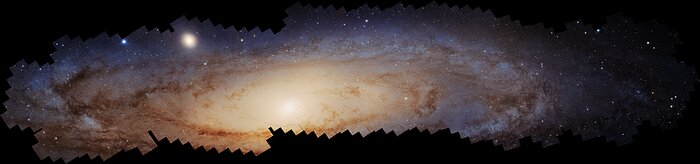
\includegraphics[width=\linewidth,height=4cm,keepaspectratio]{images/andromeda-galaxy-hubble-high-resolution--1.jpg}\par\footnotesize أندروميدا: بانوراما هابل عالية الدقة\par{\scriptsize\textcolor[HTML]{8a5a2b}{NASA, ESA, J. Dalcanton (UW)}}
\end{minipage}\hfill

\begin{minipage}{0.31\textwidth}\centering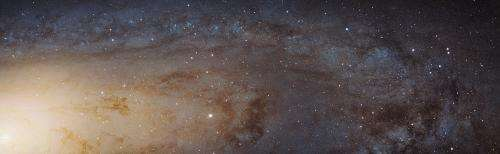
\includegraphics[width=\linewidth,height=4cm,keepaspectratio]{images/andromeda-galaxy-hubble-high-resolution--2.jpg}\par\footnotesize أندروميدا: نسخة مصغّرة من البانوراما\par{\scriptsize\textcolor[HTML]{8a5a2b}{NASA, ESA, J. Dalcanton (UW)}}
\end{minipage}\hfill

\begin{minipage}{0.31\textwidth}\centering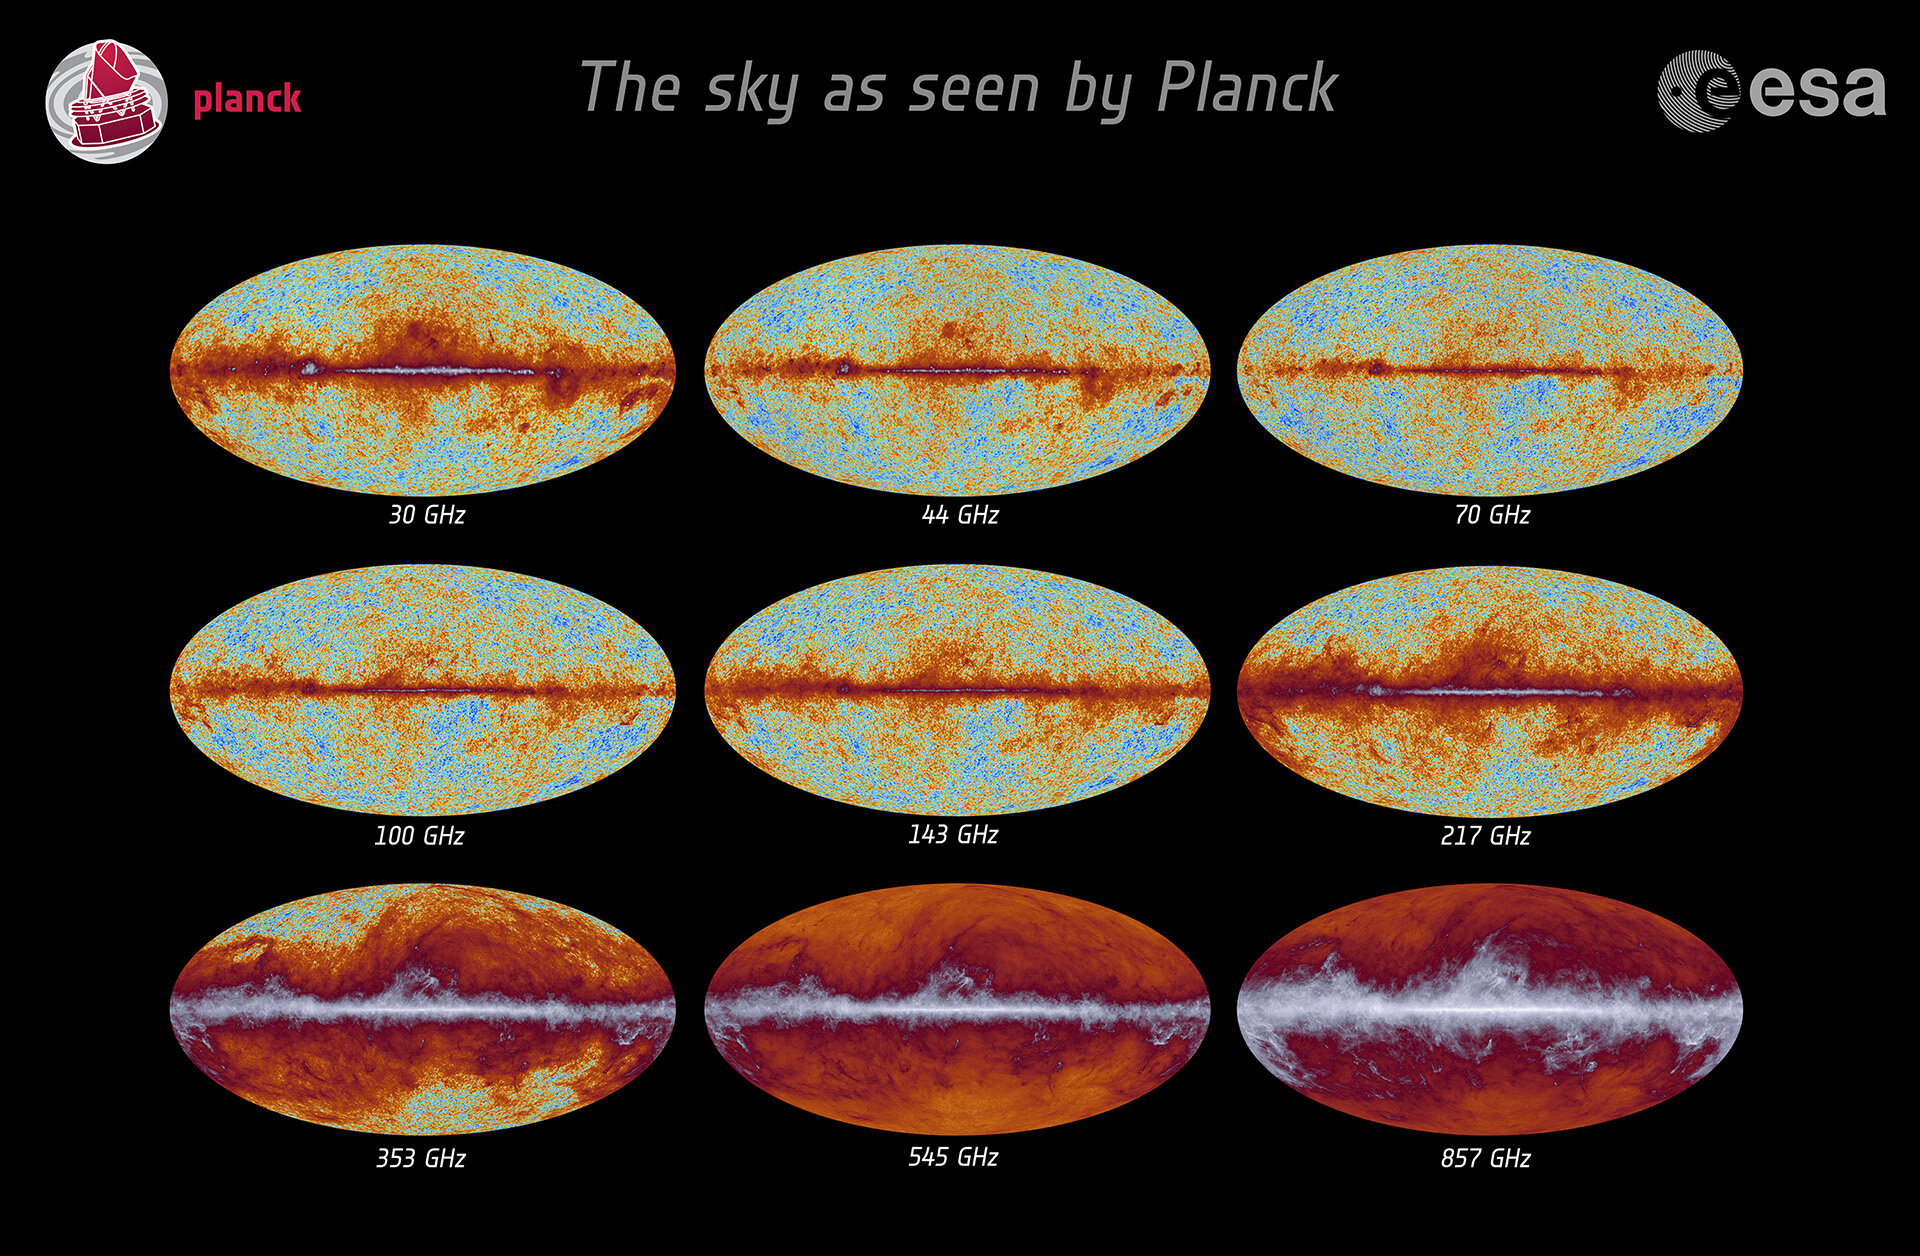
\includegraphics[width=\linewidth,height=4cm,keepaspectratio]{images/planck-cosmic-microwave-background-map-e-2.jpg}\par\footnotesize بلانك: السماء كاملةً في تسع نطاقات ترددية\par{\scriptsize\textcolor[HTML]{8a5a2b}{ESA / Planck Collaboration}}
\end{minipage}
\vspace{0.6em}

\begin{minipage}{0.31\textwidth}\centering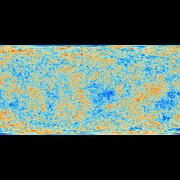
\includegraphics[width=\linewidth,height=4cm,keepaspectratio]{images/planck-cosmic-microwave-background-map-e-1.jpg}\par\footnotesize شريطُ السماء: تباينات الخلفية الميكروية\par{\scriptsize\textcolor[HTML]{8a5a2b}{ESA / Planck Collaboration}}
\end{minipage}\hfill

\begin{minipage}{0.31\textwidth}\centering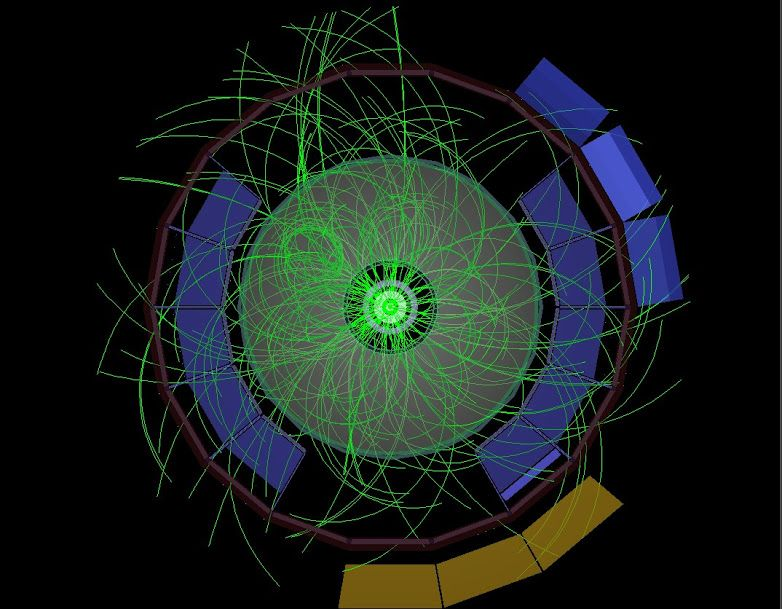
\includegraphics[width=\linewidth,height=4cm,keepaspectratio]{images/alice-detector-lead-ion-collision-quark--2.jpg}\par\footnotesize ALICE: تصادم أيونات الرصاص\par{\scriptsize\textcolor[HTML]{8a5a2b}{CERN / ALICE}}
\end{minipage}\hfill

\begin{minipage}{0.31\textwidth}\centering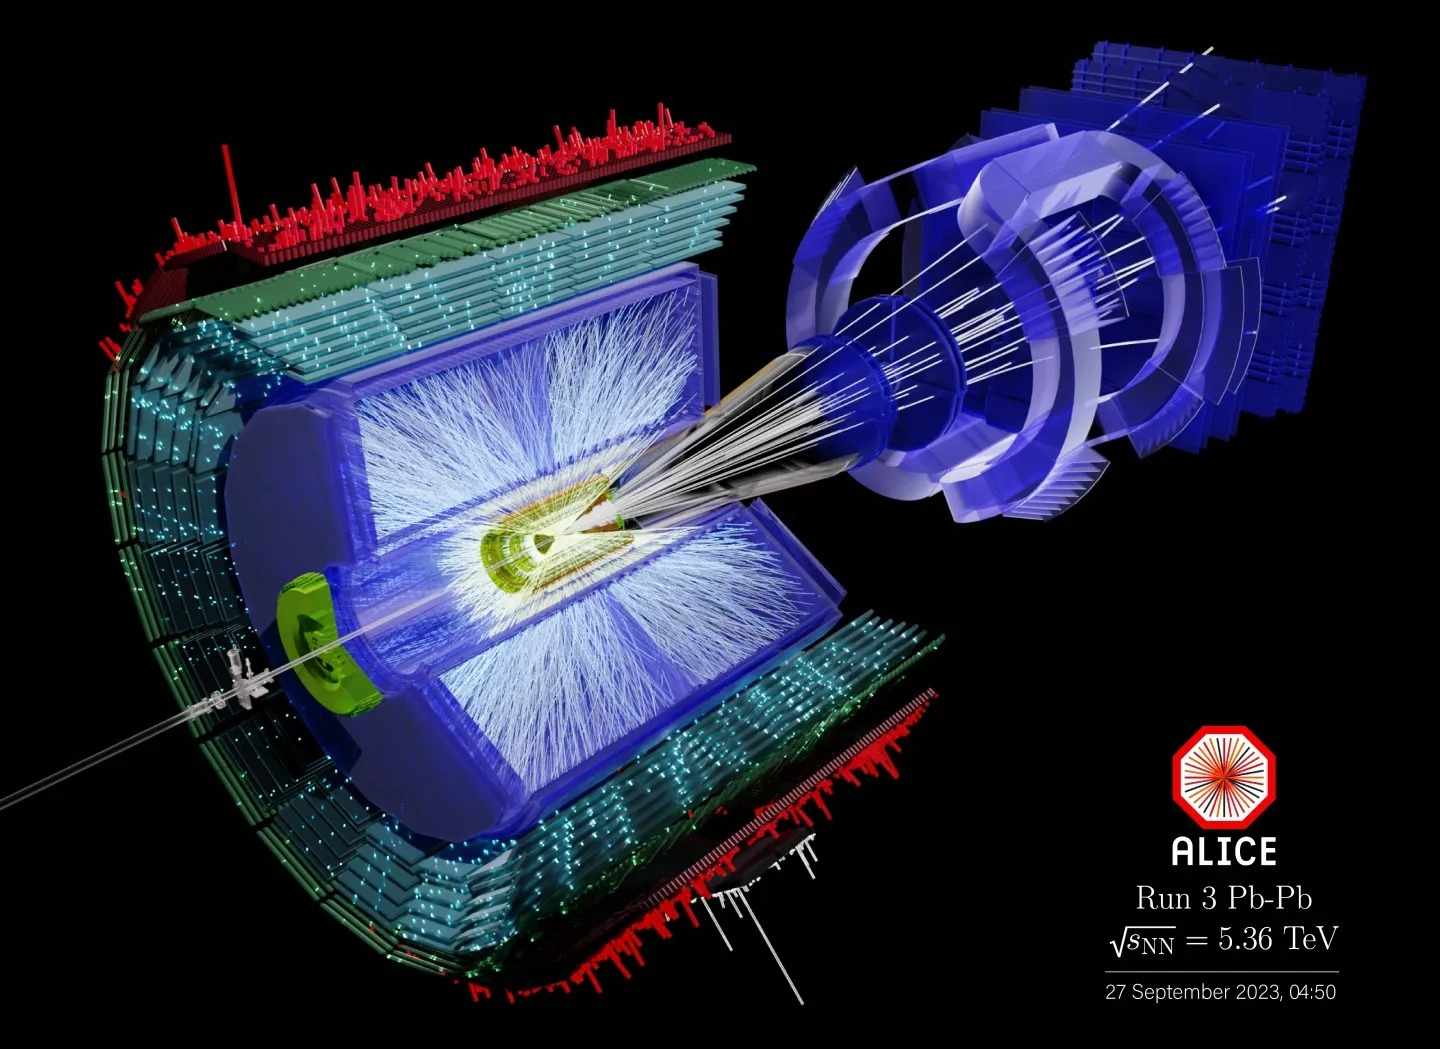
\includegraphics[width=\linewidth,height=4cm,keepaspectratio]{images/alice-detector-lead-ion-collision-quark--1.jpg}\par\footnotesize ALICE: مقطعٌ في الكاشف\par{\scriptsize\textcolor[HTML]{8a5a2b}{CERN / ALICE}}
\end{minipage}
\vspace{0.6em}

\begin{minipage}{0.31\textwidth}\centering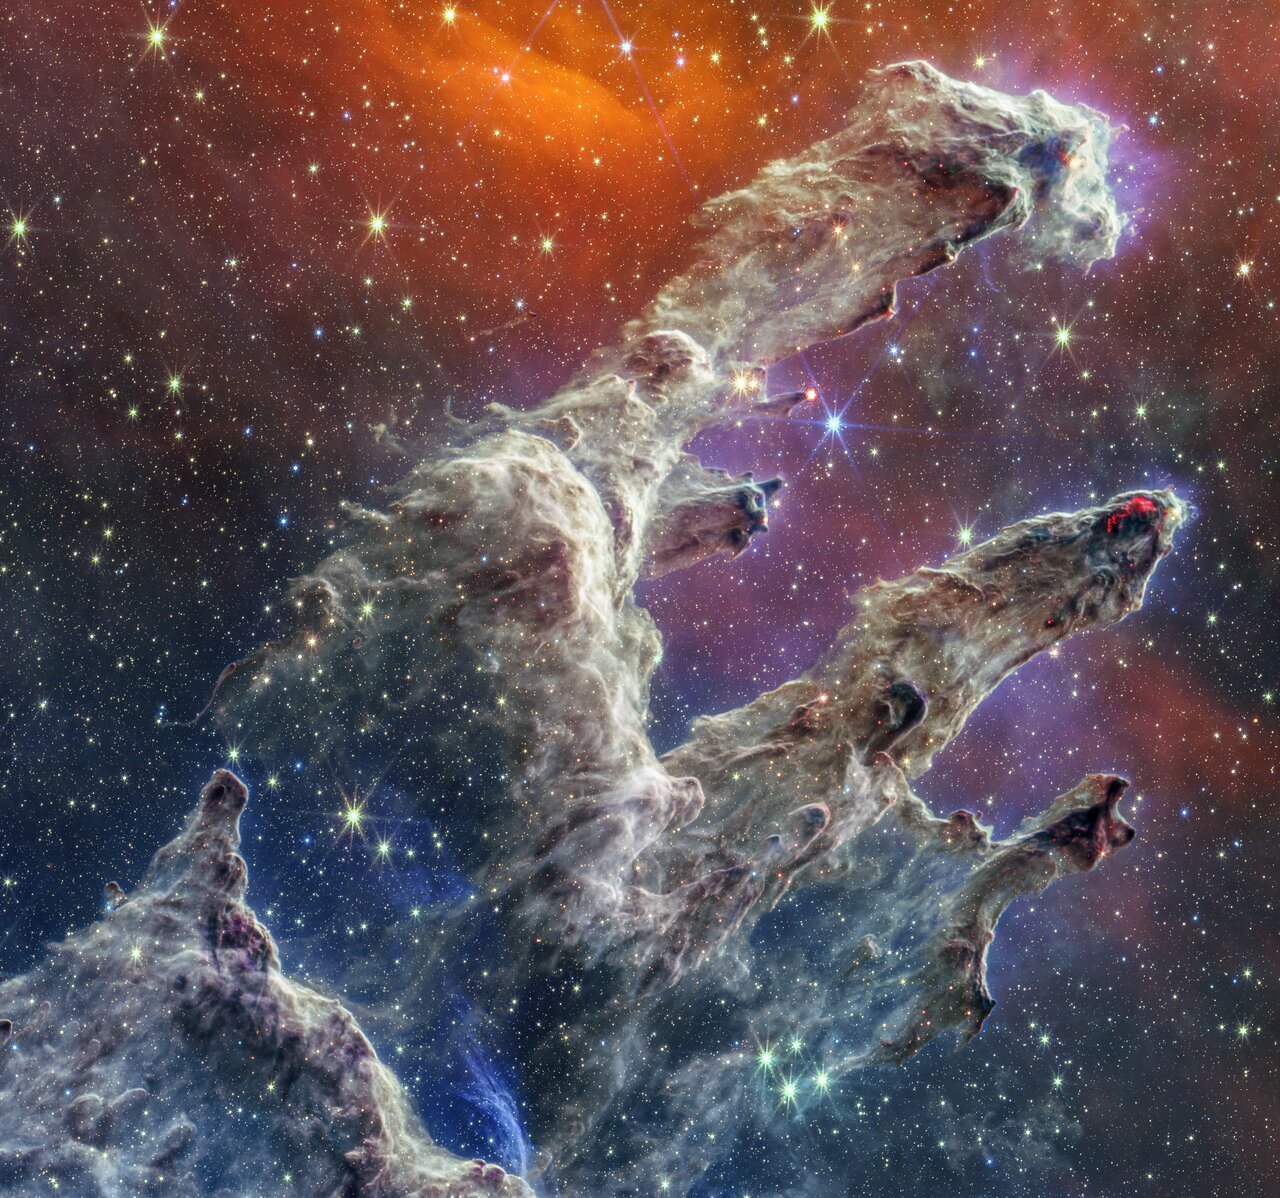
\includegraphics[width=\linewidth,height=4cm,keepaspectratio]{images/jwst-pillars-of-creation-carina-nebula-i-1.jpg}\par\footnotesize أعمدة الخلق — جيمس ويب\par{\scriptsize\textcolor[HTML]{8a5a2b}{NASA, ESA, CSA, STScI}}
\end{minipage}\hfill

\begin{minipage}{0.31\textwidth}\centering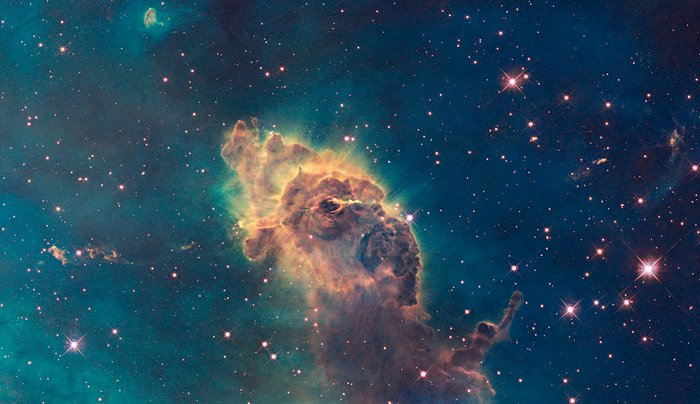
\includegraphics[width=\linewidth,height=4cm,keepaspectratio]{images/jwst-pillars-of-creation-carina-nebula-i-2.jpg}\par\footnotesize القاعدة — هابل ٢٠٠٩\par{\scriptsize\textcolor[HTML]{8a5a2b}{NASA, ESA, Hubble Heritage}}
\end{minipage}\hfill

\begin{minipage}{0.31\textwidth}\centering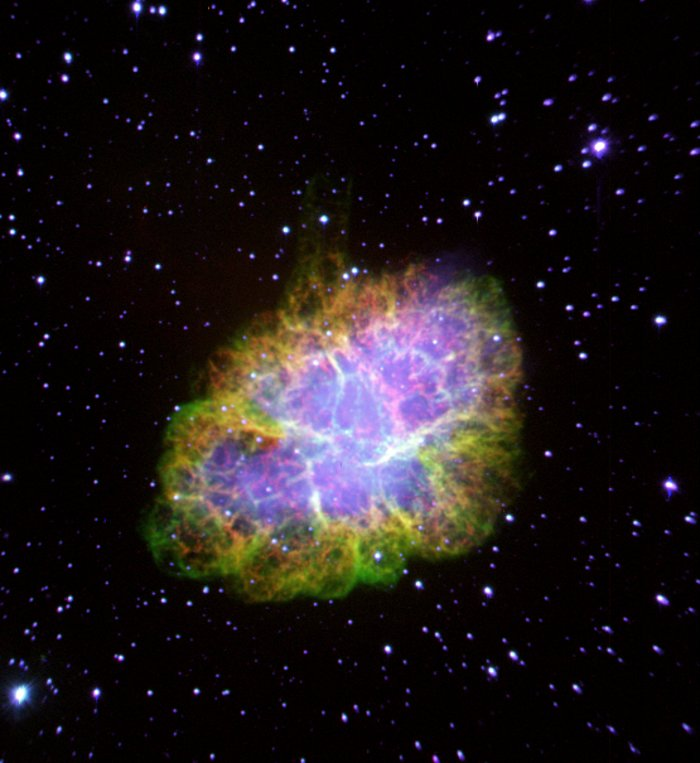
\includegraphics[width=\linewidth,height=4cm,keepaspectratio]{images/crab-nebula-supernova-remnant-hubble-spa-2.jpg}\par\footnotesize السرطان: بقايا مستعر ١٠٥٤\par{\scriptsize\textcolor[HTML]{8a5a2b}{NASA, ESA, J. Hester \& A. Loll}}
\end{minipage}
\vspace{0.6em}

\begin{minipage}{0.31\textwidth}\centering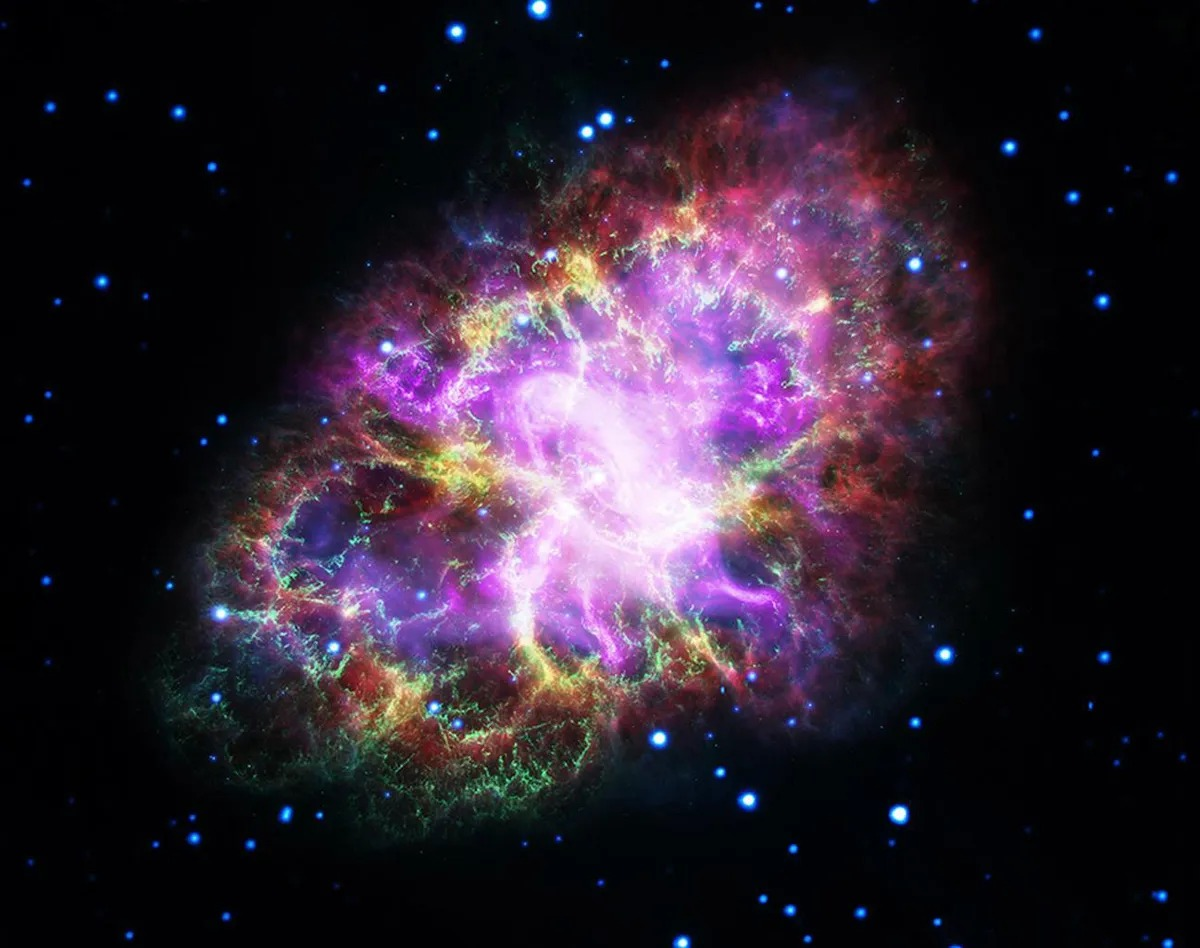
\includegraphics[width=\linewidth,height=4cm,keepaspectratio]{images/crab-nebula-supernova-remnant-hubble-spa-1.jpg}\par\footnotesize السرطان بأطوال موجية متعددة\par{\scriptsize\textcolor[HTML]{8a5a2b}{NASA, ESA, G. Dubner}}
\end{minipage}\hfill

\begin{minipage}{0.31\textwidth}\centering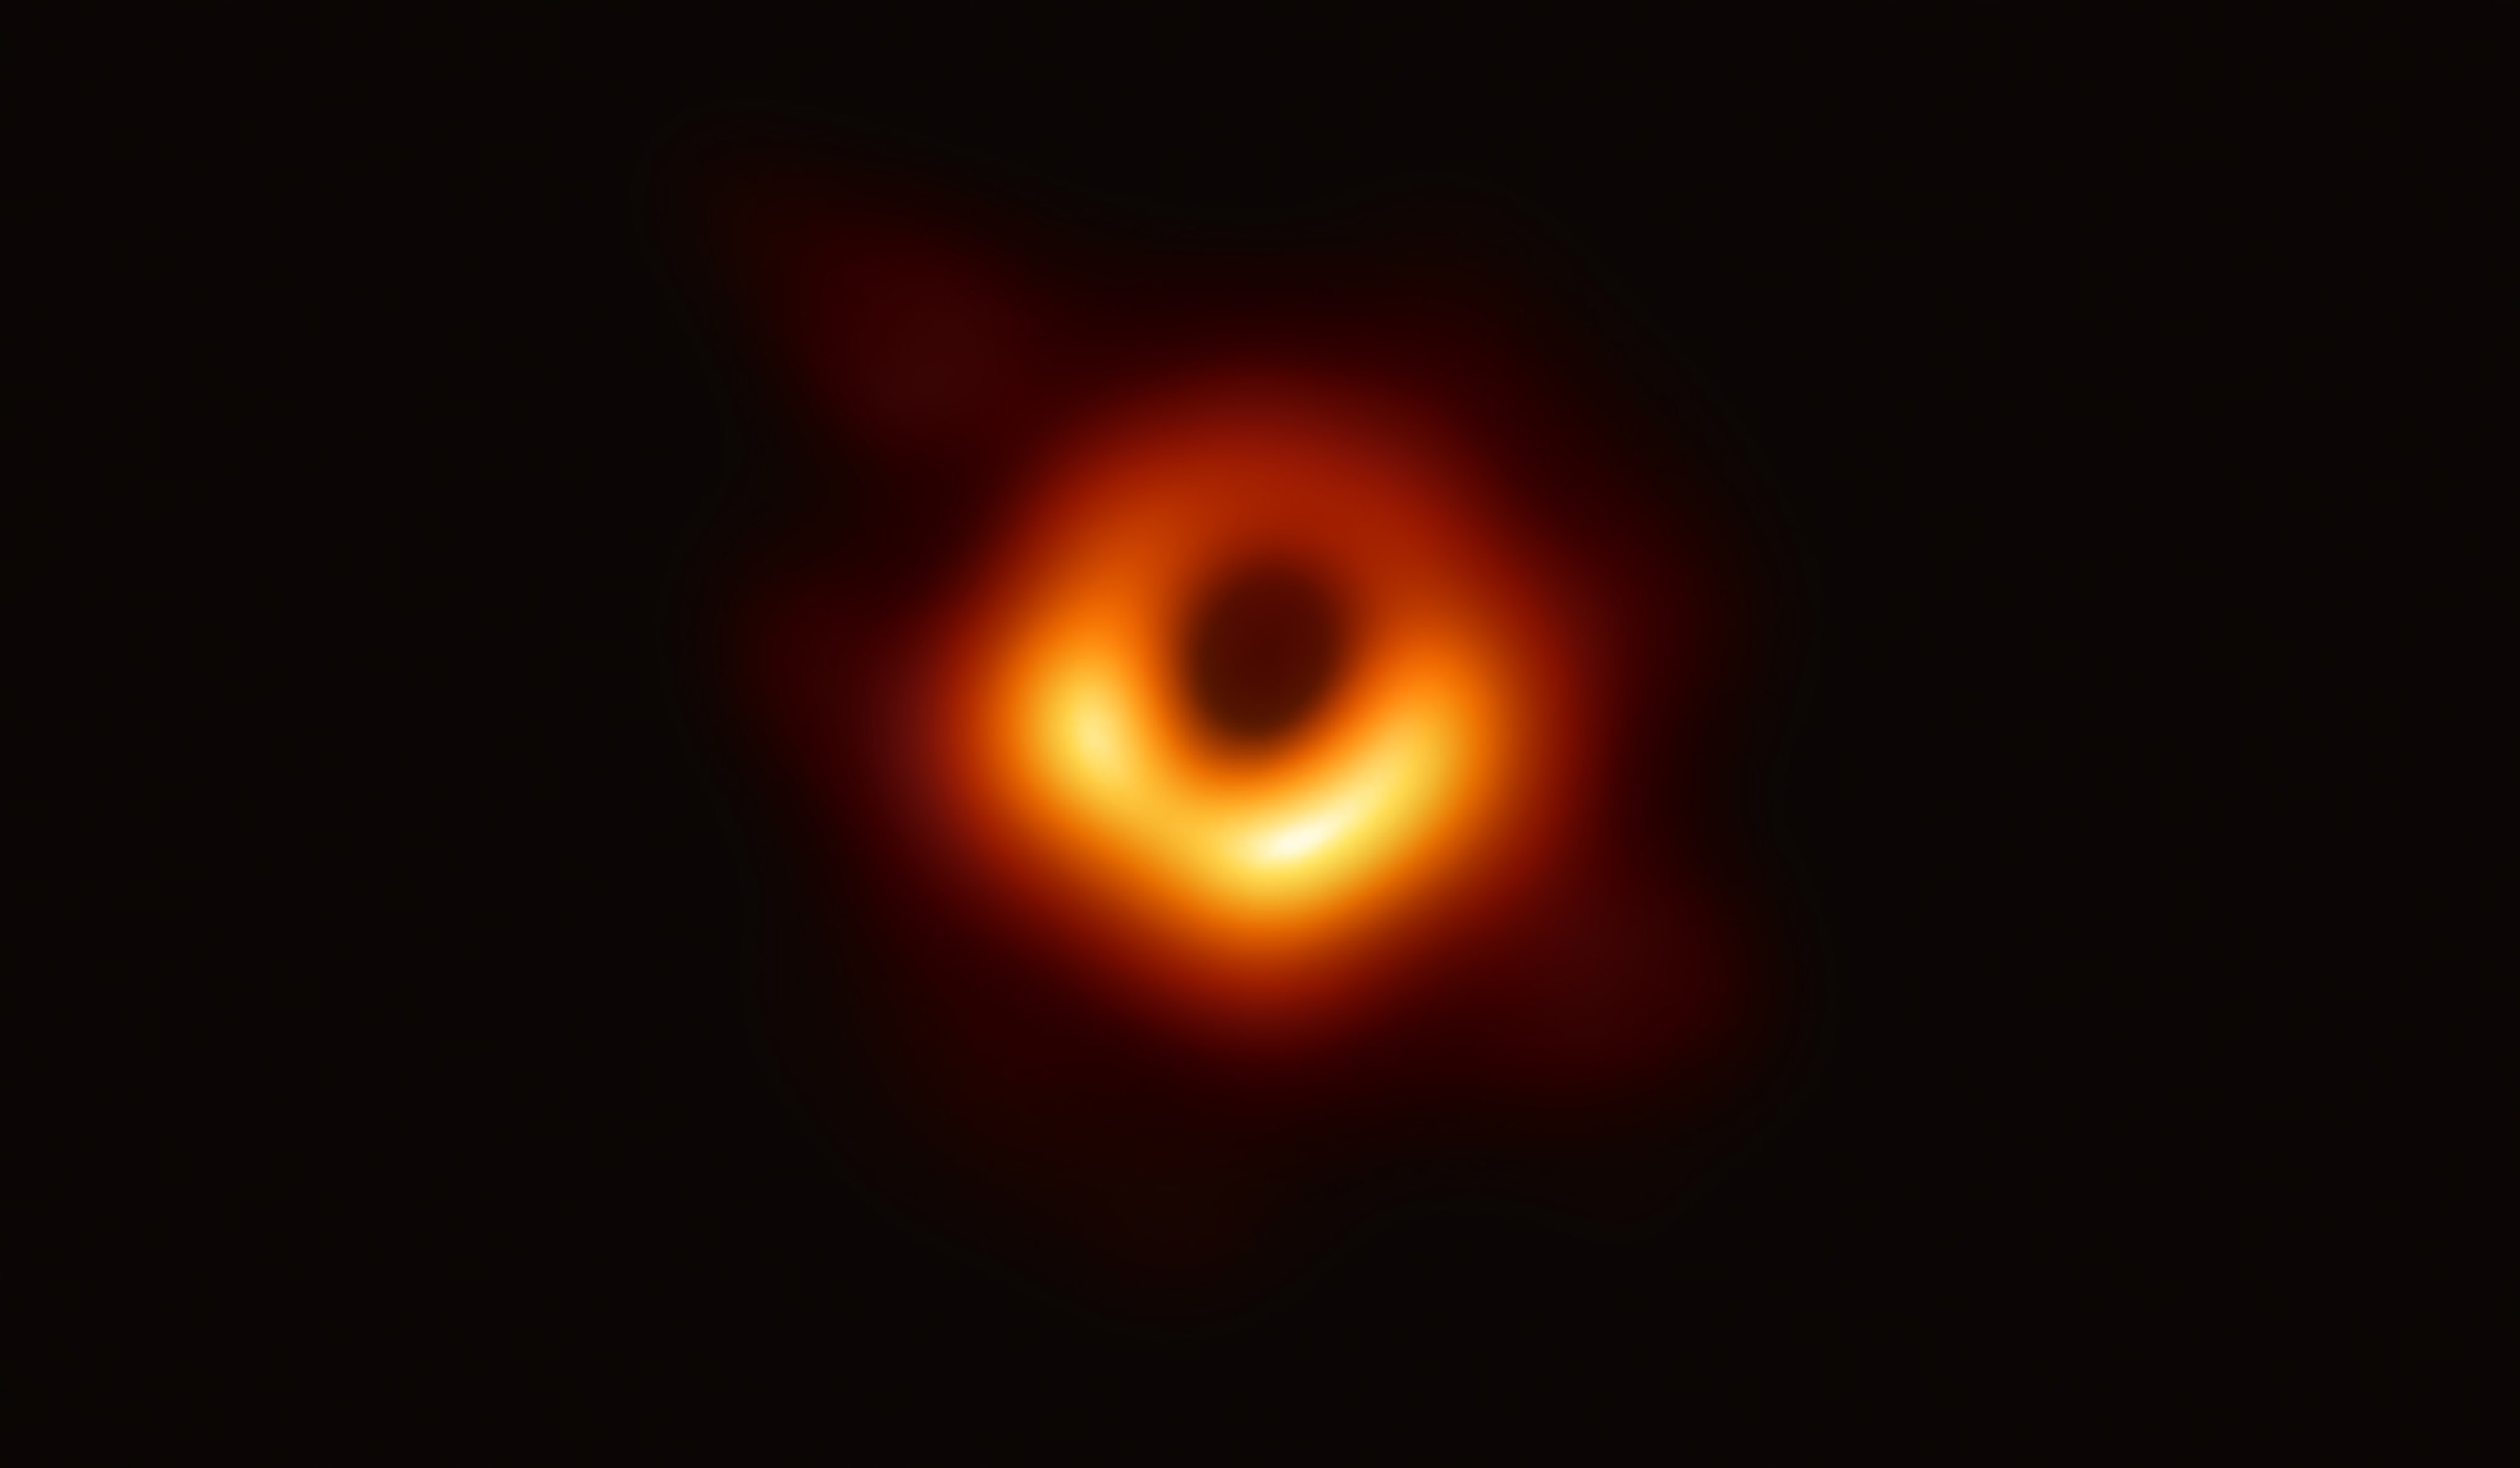
\includegraphics[width=\linewidth,height=4cm,keepaspectratio]{images/event-horizon-telescope-first-image-m87--1.jpg}\par\footnotesize M87*: أول صورة لظلّ ثقب أسود\par{\scriptsize\textcolor[HTML]{8a5a2b}{EHT Collaboration}}
\end{minipage}\hfill

\begin{minipage}{0.31\textwidth}\centering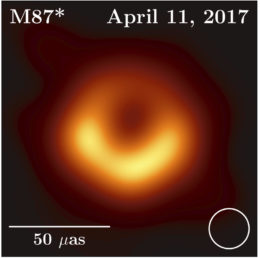
\includegraphics[width=\linewidth,height=4cm,keepaspectratio]{images/event-horizon-telescope-first-image-m87--2.jpg}\par\footnotesize M87*: الصورة مع الحلقة المؤشَّرة\par{\scriptsize\textcolor[HTML]{8a5a2b}{EHT Collaboration}}
\end{minipage}
\vspace{0.6em}

\begin{minipage}{0.31\textwidth}\centering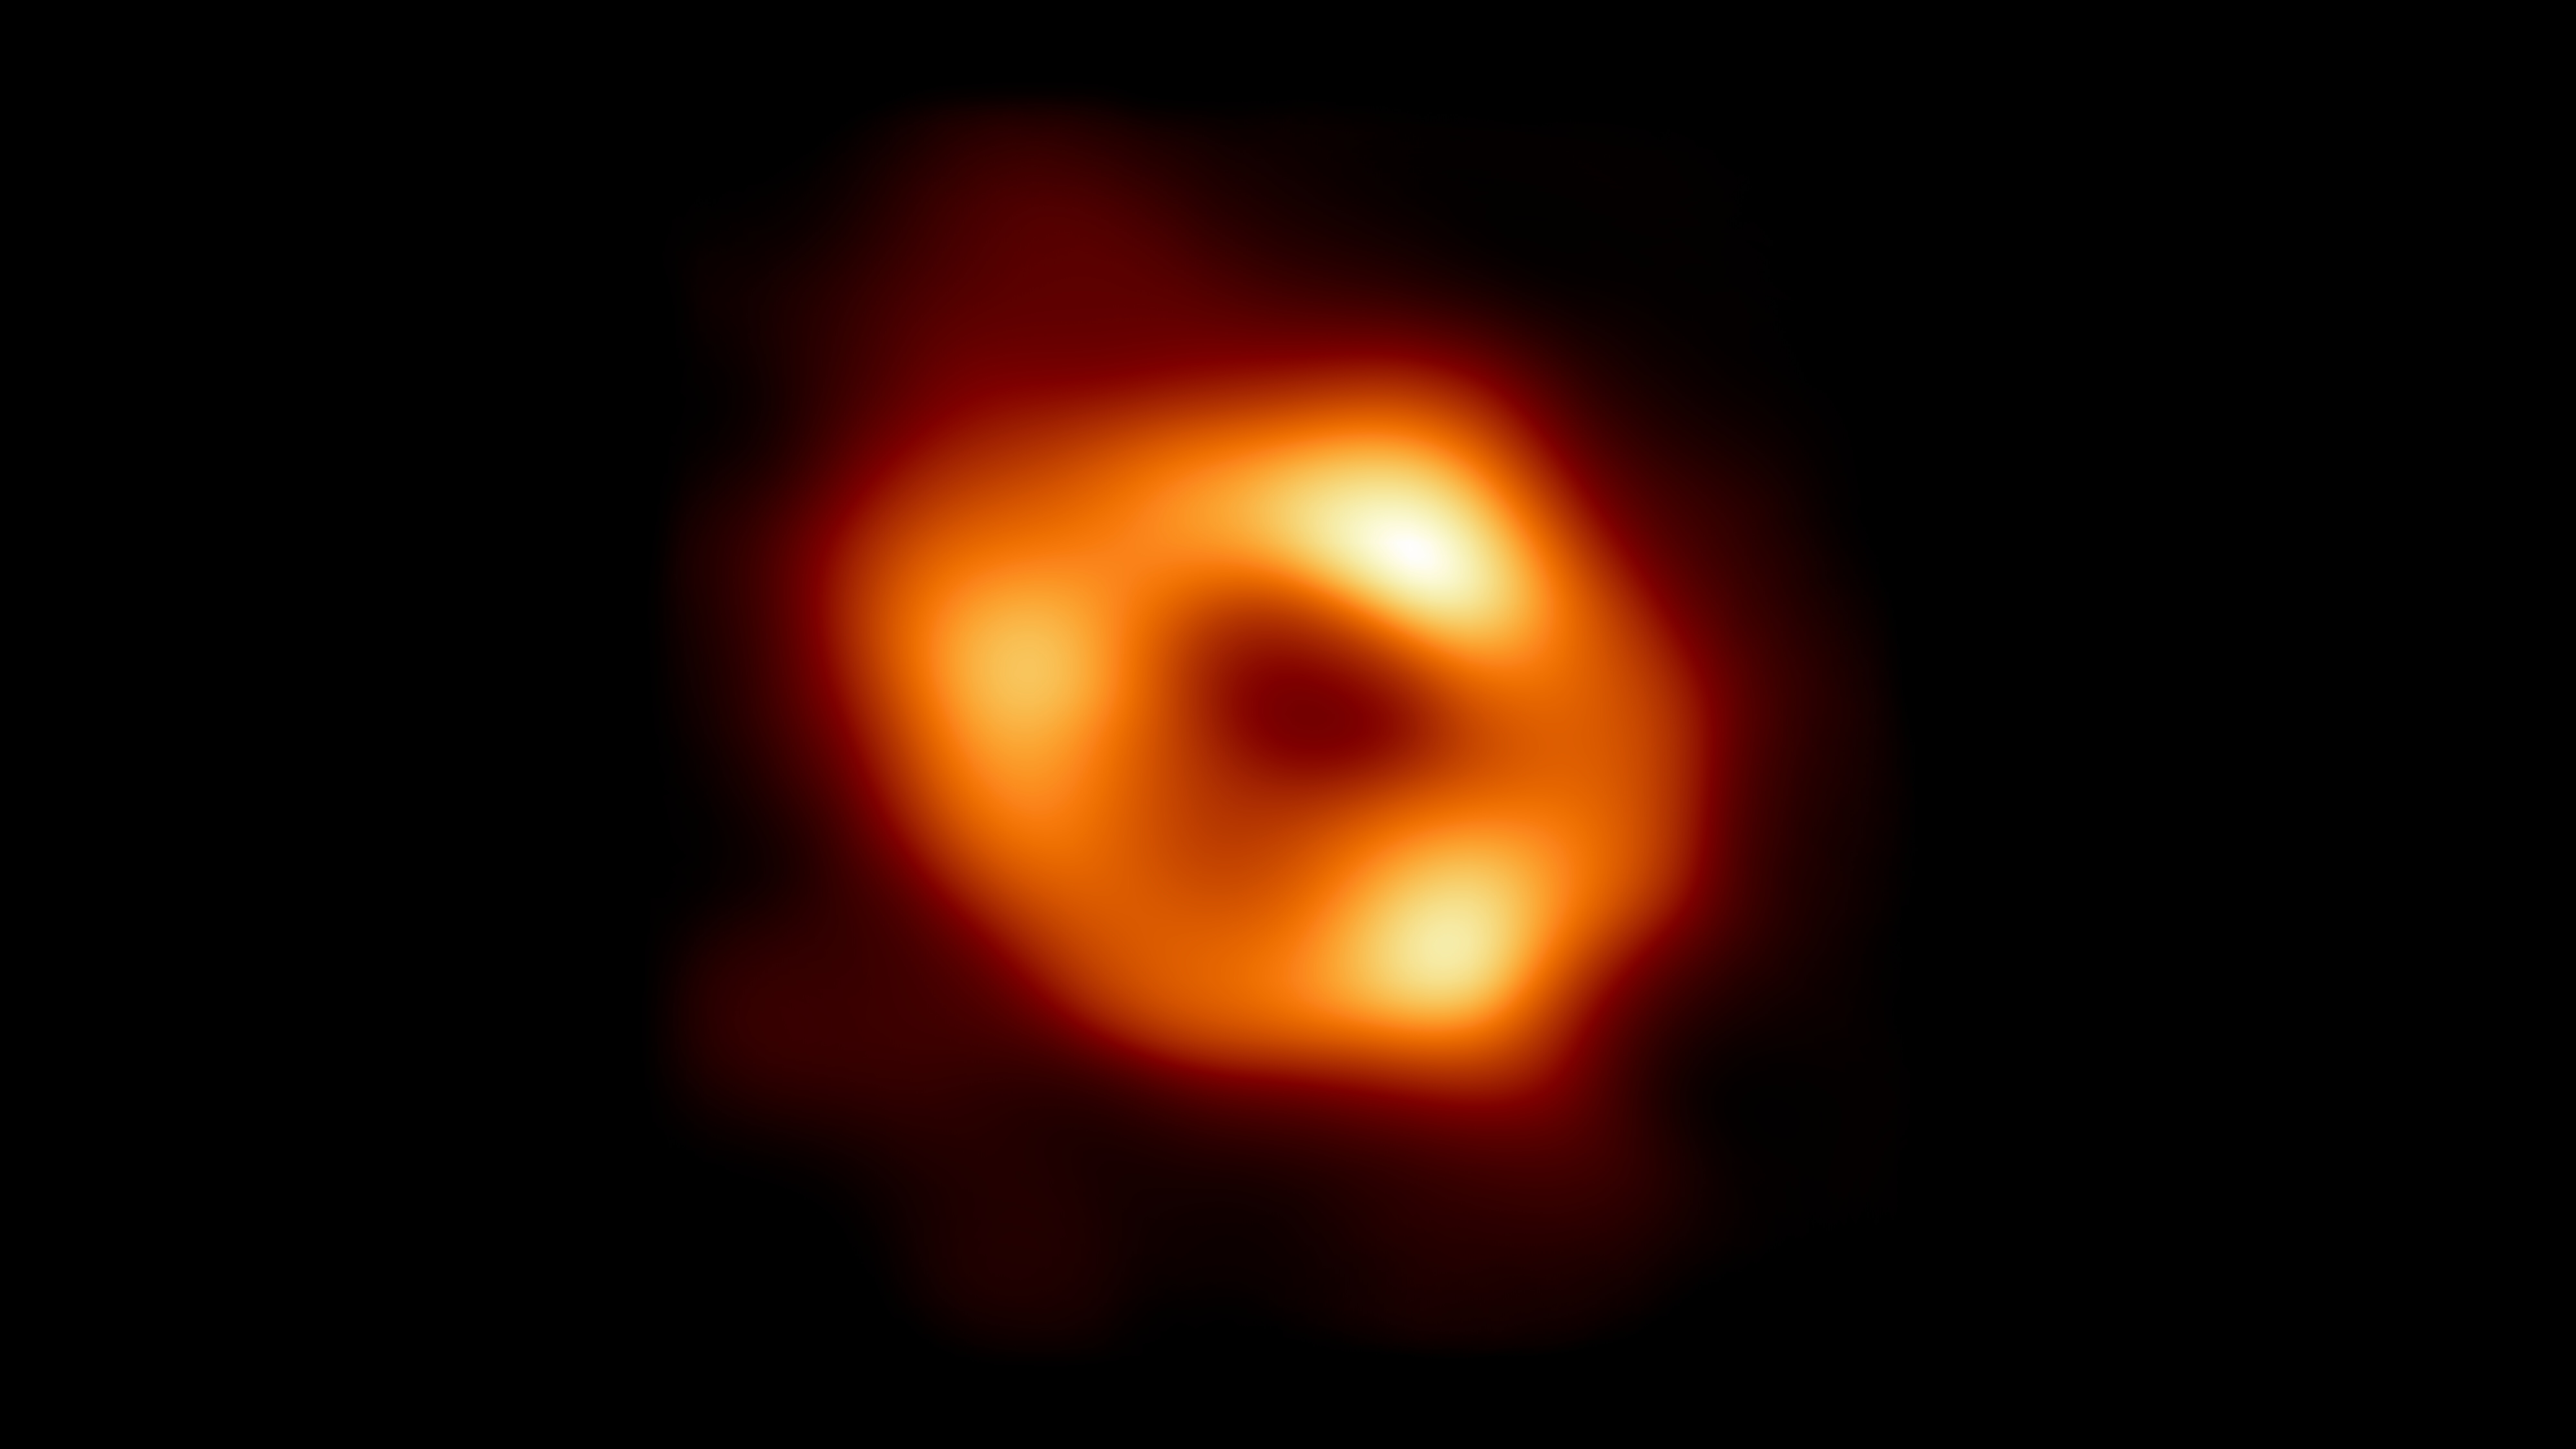
\includegraphics[width=\linewidth,height=4cm,keepaspectratio]{images/sagittarius-a-event-horizon-telescope-im-1.jpg}\par\footnotesize ساجيتاريوس A* — تلسكوب أفق الحدث\par{\scriptsize\textcolor[HTML]{8a5a2b}{EHT Collaboration}}
\end{minipage}\hfill

\begin{minipage}{0.31\textwidth}\centering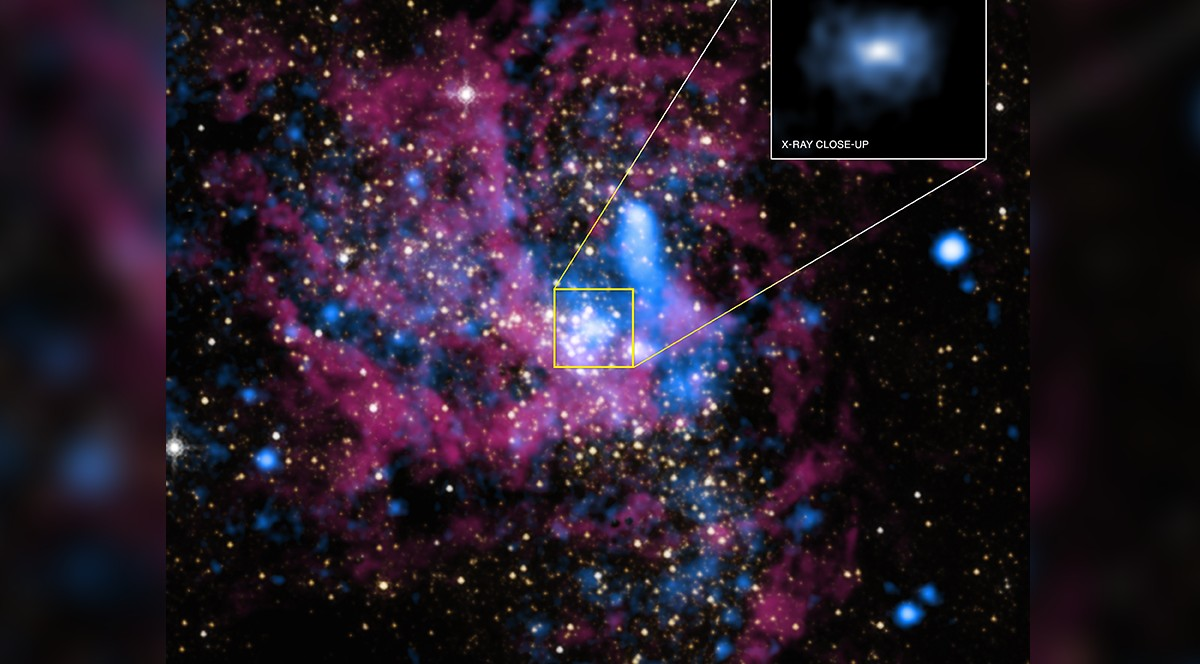
\includegraphics[width=\linewidth,height=4cm,keepaspectratio]{images/sagittarius-a-event-horizon-telescope-im-2.jpg}\par\footnotesize مركز المجرّة — شاندرا (أشعة سينية)\par{\scriptsize\textcolor[HTML]{8a5a2b}{NASA / CXC}}
\end{minipage}\hfill

\begin{minipage}{0.31\textwidth}\centering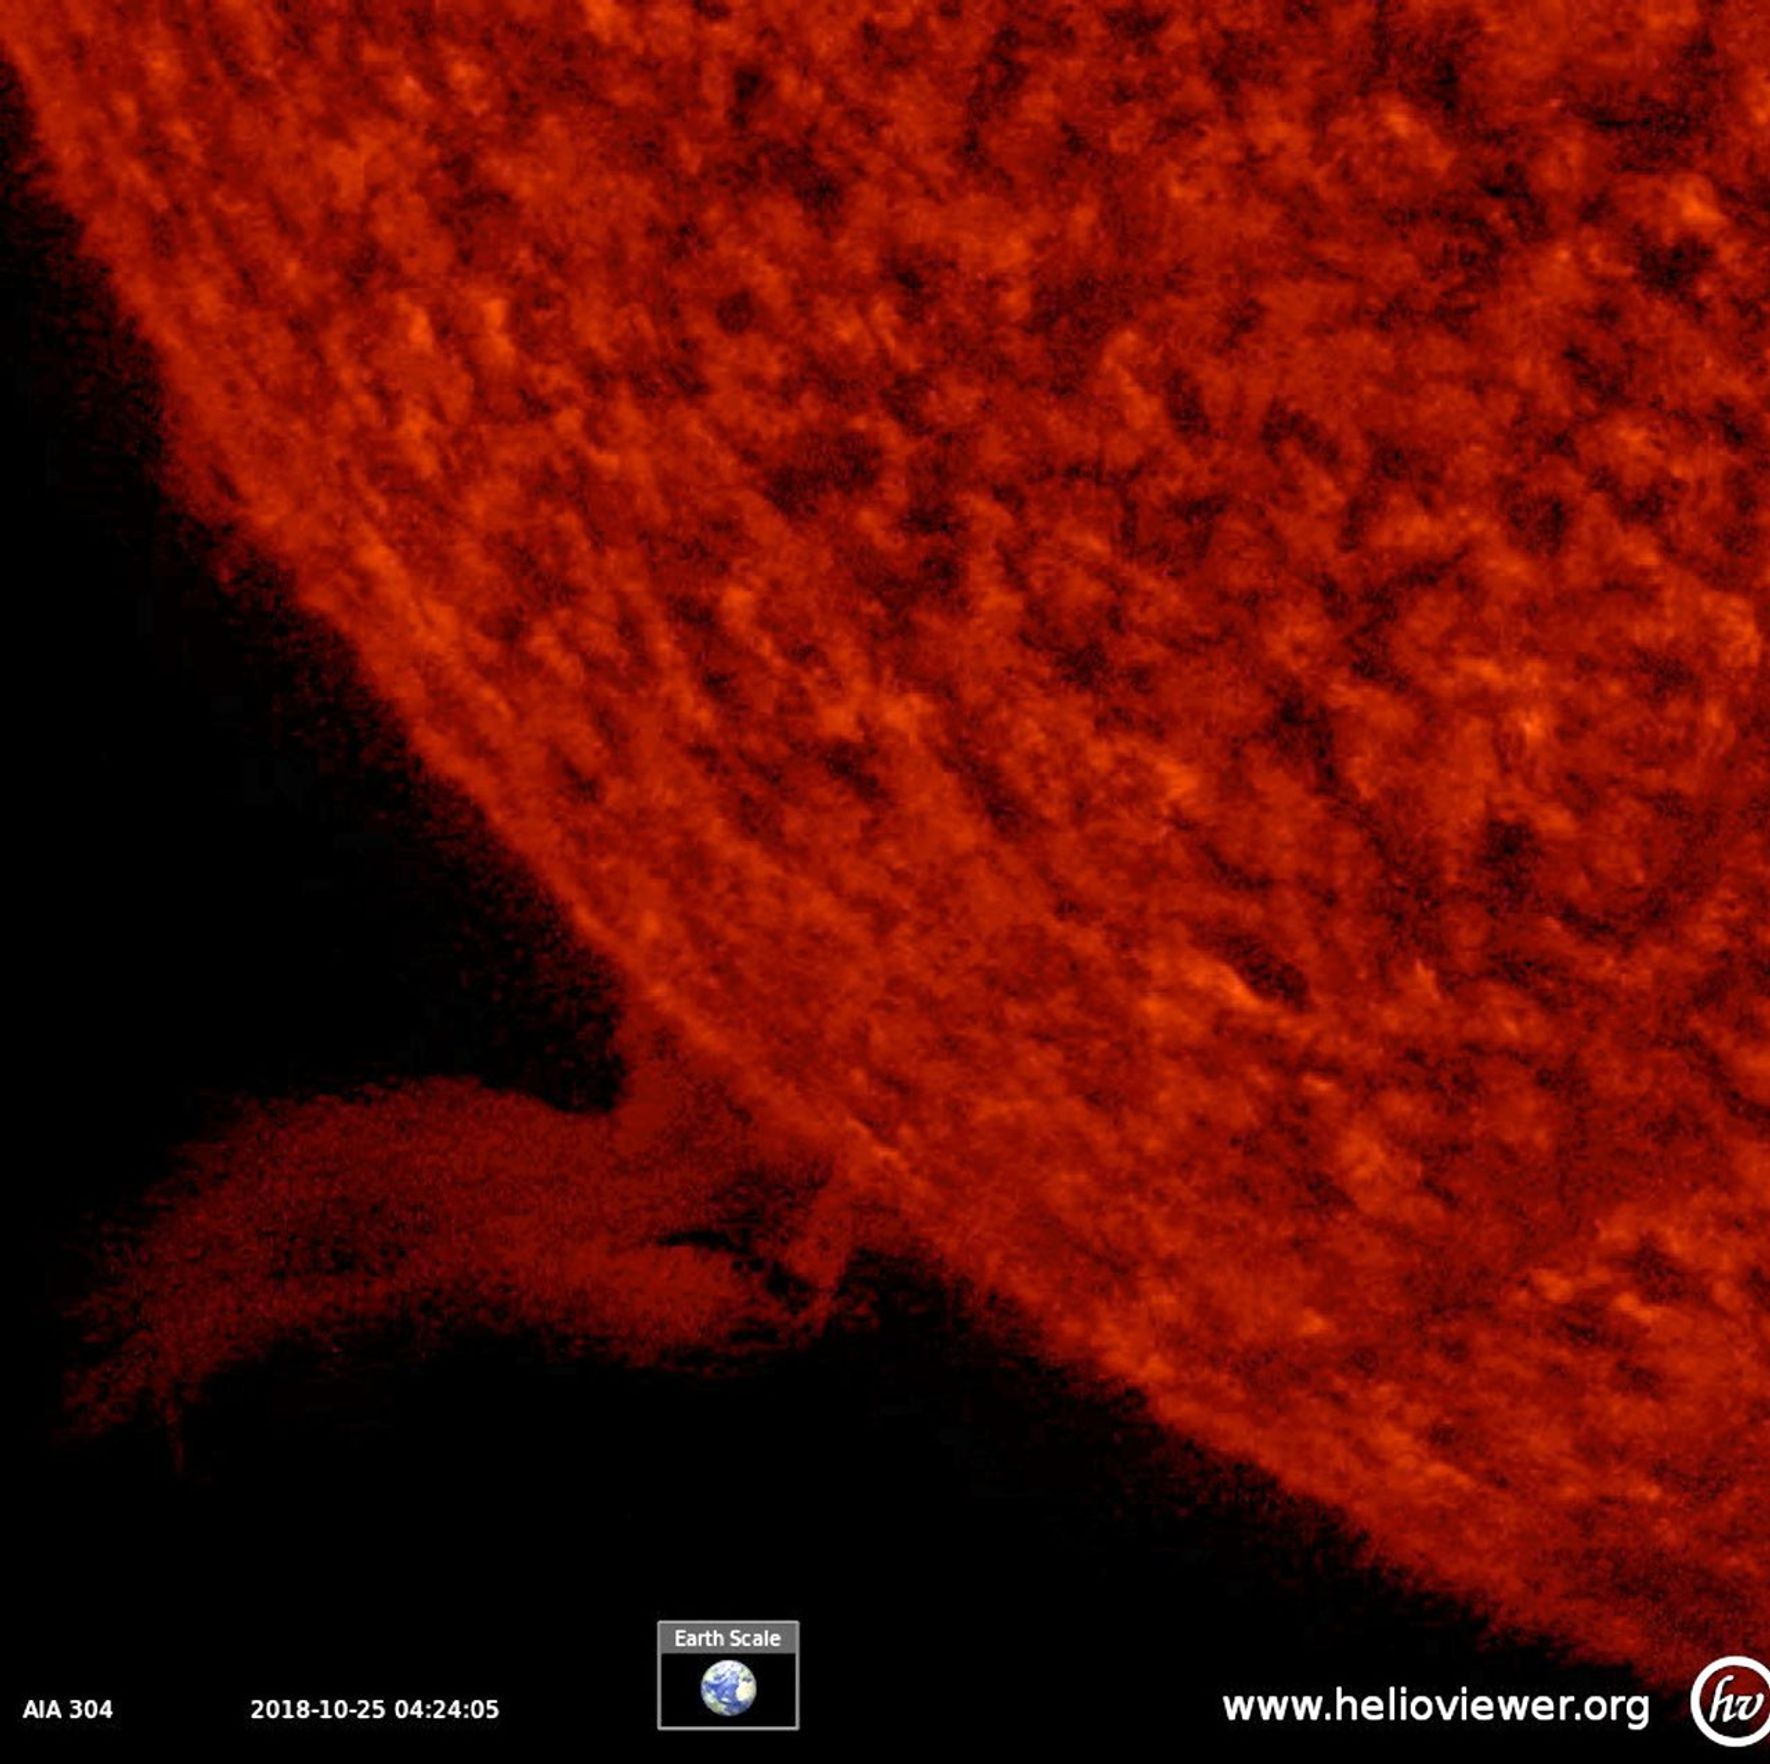
\includegraphics[width=\linewidth,height=4cm,keepaspectratio]{images/solar-prominence-solar-dynamics-observat-1.jpg}\par\footnotesize اندفاعٌ شمسي — SDO\par{\scriptsize\textcolor[HTML]{8a5a2b}{NASA / SDO}}
\end{minipage}
\vspace{0.6em}

\begin{minipage}{0.31\textwidth}\centering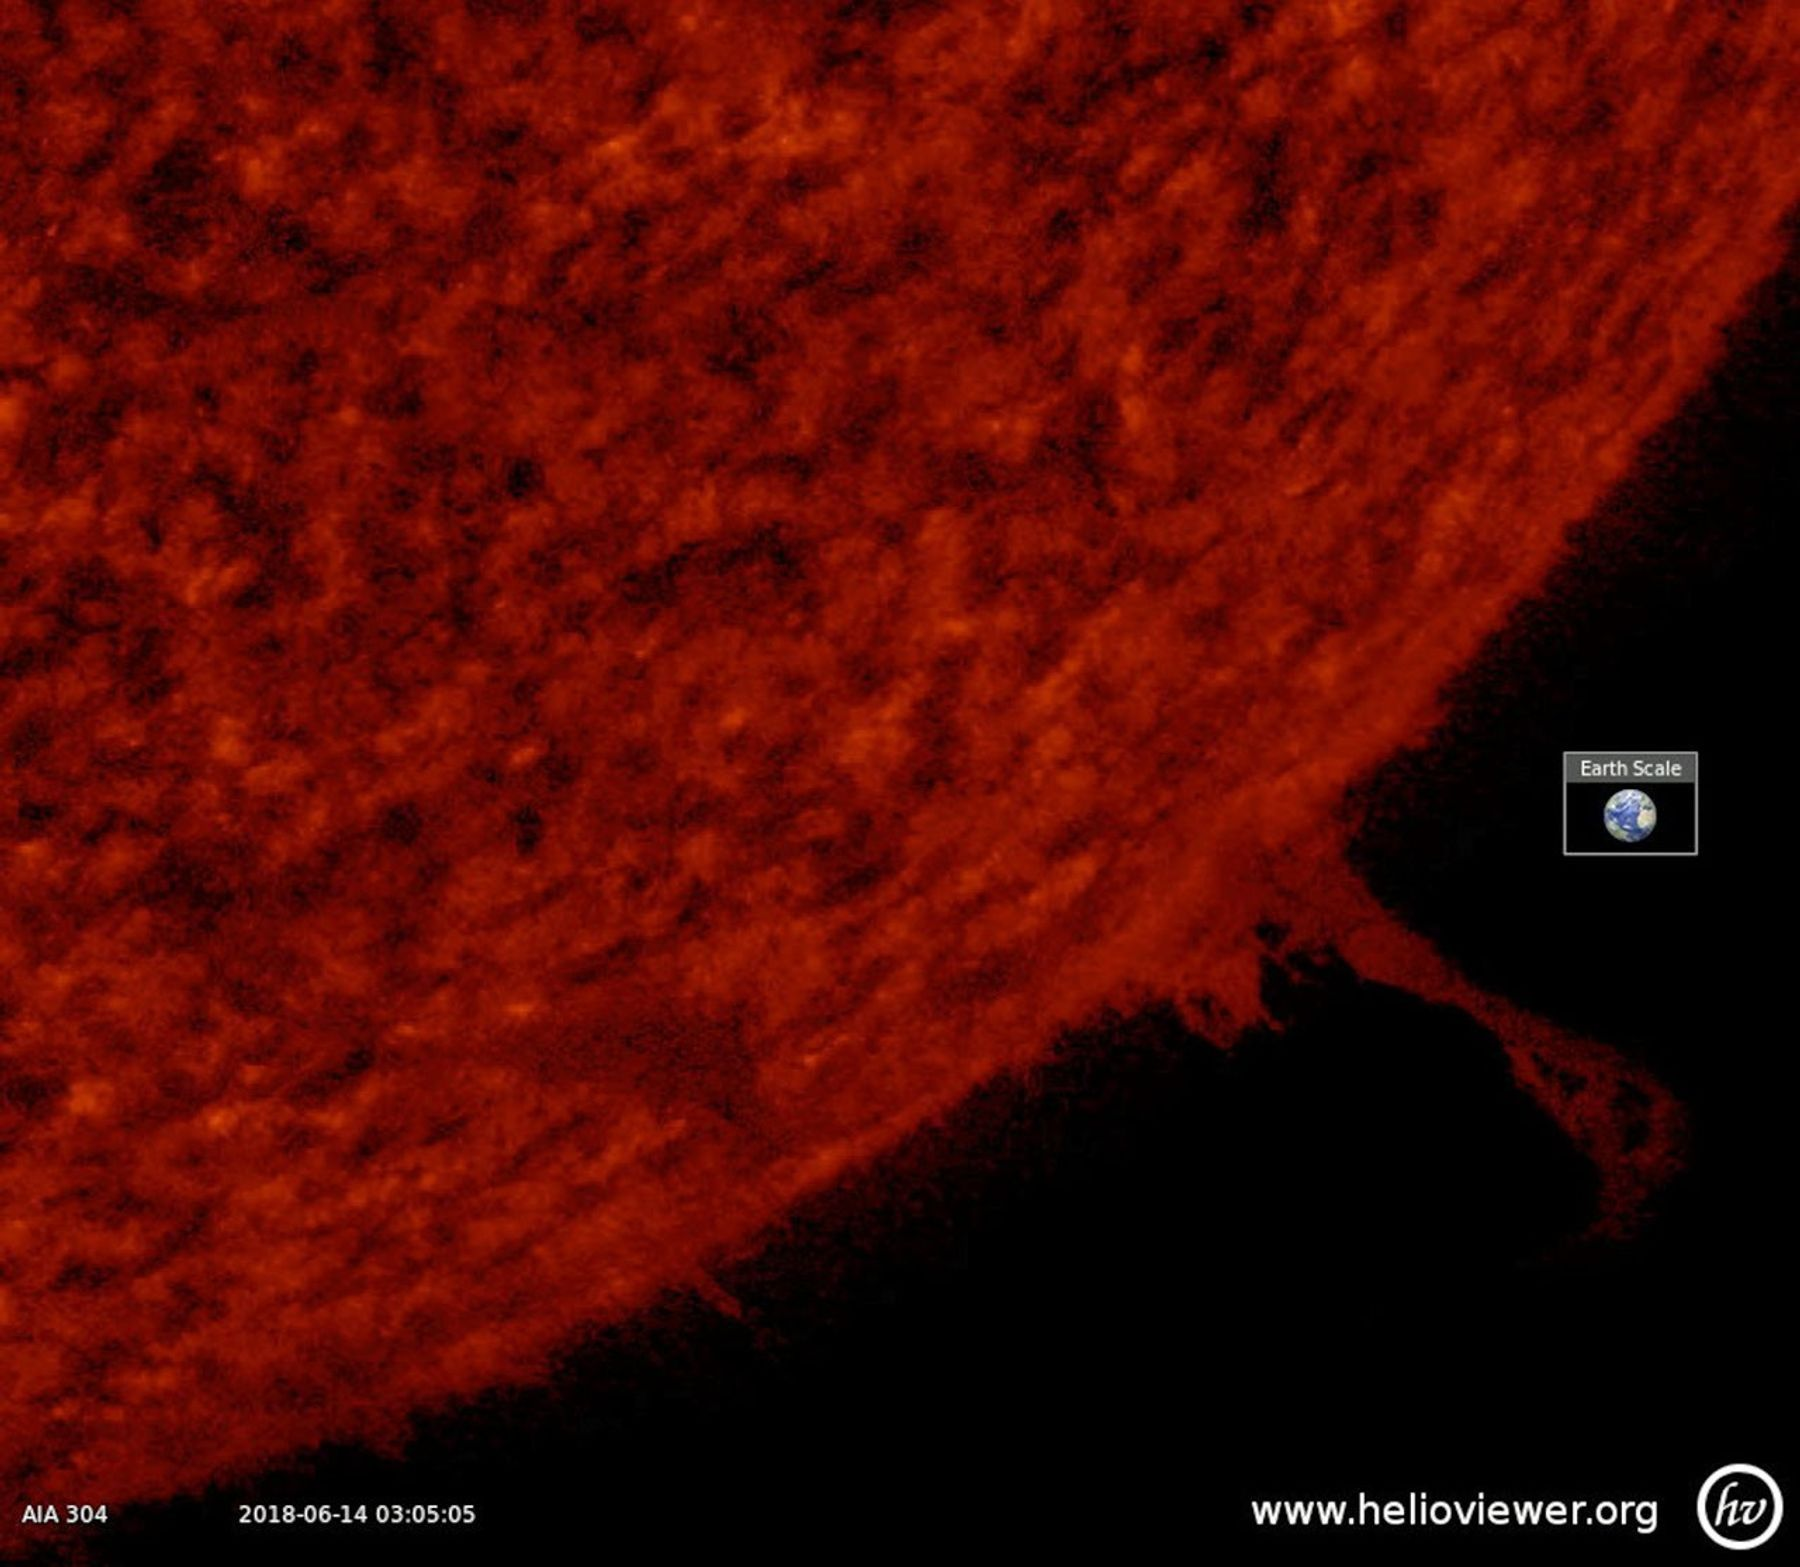
\includegraphics[width=\linewidth,height=4cm,keepaspectratio]{images/solar-prominence-solar-dynamics-observat-2.jpg}\par\footnotesize شُوَاظٌ متطوّر — SDO\par{\scriptsize\textcolor[HTML]{8a5a2b}{NASA / SDO}}
\end{minipage}\hfill

\begin{minipage}{0.31\textwidth}\centering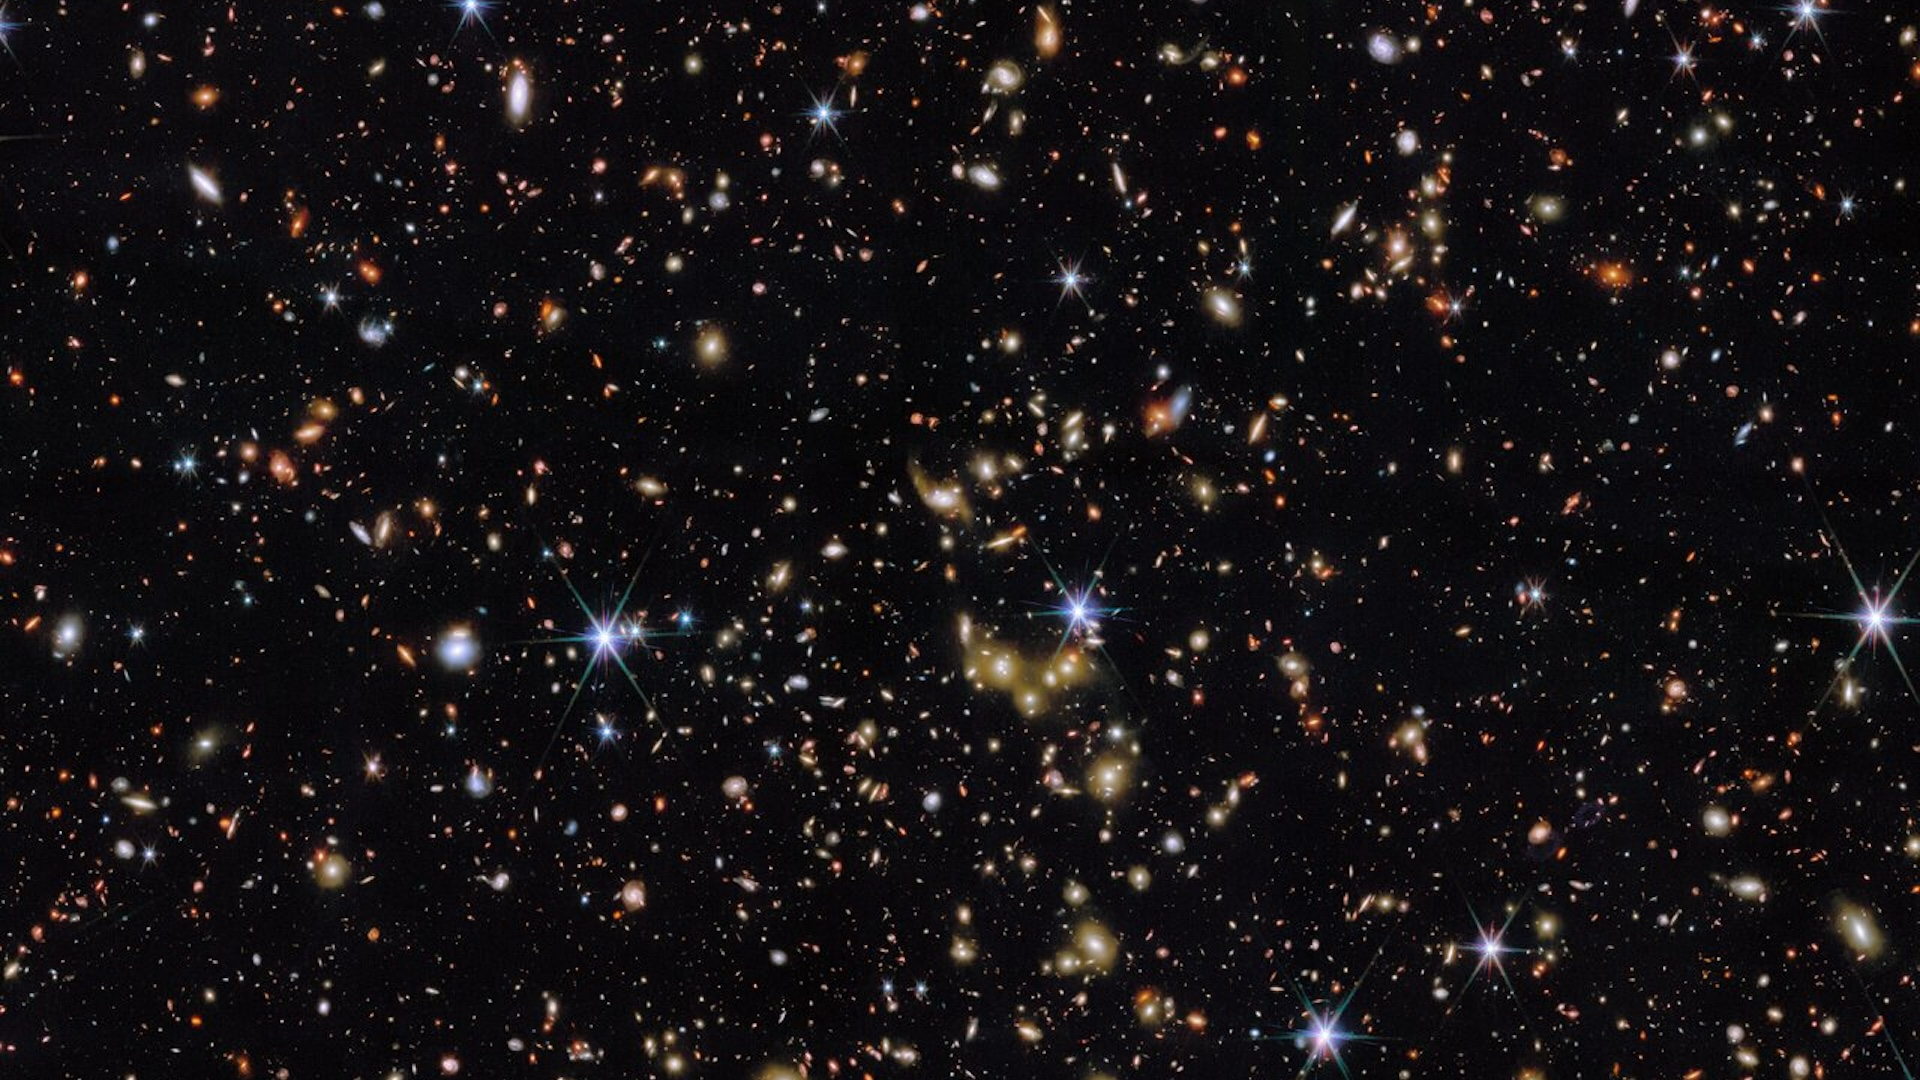
\includegraphics[width=\linewidth,height=4cm,keepaspectratio]{images/james-webb-space-telescope-deep-field-th-1.jpg}\par\footnotesize حقل جيمس ويب العميق\par{\scriptsize\textcolor[HTML]{8a5a2b}{NASA, ESA, CSA, STScI}}
\end{minipage}\hfill

\begin{minipage}{0.31\textwidth}\centering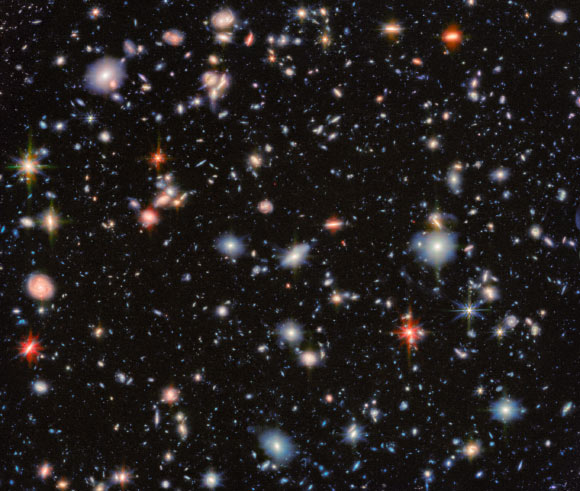
\includegraphics[width=\linewidth,height=4cm,keepaspectratio]{images/james-webb-space-telescope-deep-field-th-2.jpg}\par\footnotesize حقل ويب العميق — نسخة ثانية\par{\scriptsize\textcolor[HTML]{8a5a2b}{NASA, ESA, CSA, STScI}}
\end{minipage}
\vspace{0.6em}

\end{figure}


\chapter*{إسناد الصور والمصادر}

أُعدّ هذا الكتاب العربي اعتماداً على النصّ الإنجليزي المنقّح «The Complete History of the Universe»، وهو نصٌّ خضع لتدقيقٍ صارم في ٥٥ موضعاً قبل الترجمة. ولم تُترجم الصور ولا أسماؤها: نُقلت كما هي من أرشيف الجهة التي أنتجتها، وأُثبت اسم الجهة في تذييل كل صورة، لأن الصورة الرصدية وثيقةٌ لها مؤلّفٌ ومصدر.


جميع الصور في هذا الكتاب ملكٌ لعامة الناس، وتُنشر بموجب سياسات النشر المعلنة لدى الوكالات المذكورة أدناه. وحيث كانت الصورة المتاحة نسخةً مصغّرة من الأصل (thumbnail)، فقد أُدرجت كما وُجدت دون تحسينٍ يُوهم بدقّةٍ أعلى.


أما النصوص فهي من كتابة النسخة العربية، ولم تُستخدم ترجمةٌ آلية في صياغتها؛ وقد رُوعي في كل جملة أن تحمل معلومةً قابلةً للتحقّق: رقماً أو تاريخاً أو نتيجةَ رصد.


\begin{description}

\item[NASA] أرشيف الصور العلمية · الشمس، شاندرا، هابل

\item[ESA / Hubble] أرشيف هابل الأوروبي · أندروميدا، القاعدة، السرطان

\item[NASA, ESA, CSA, STScI] تلسكوب جيمس ويب · الحقول العميقة وأعمدة الخلق

\item[ESA / Planck] خريطة الخلفية الميكروية · ٢٠١٣–٢٠١٨

\item[EHT Collaboration] تلسكوب أفق الحدث · M87* وساجيتاريوس A*

\item[CERN / ALICE] كاشف ALICE · تصادمات أيونات الرصاص

\end{description}


\vfill\begin{center}\large تمّ بحمد الله\end{center}


\end{document}
